\documentclass[11pt,a4paper]{report}

% ---------- packages ----------
\usepackage[utf8]{inputenc}
\usepackage[T1]{fontenc}
\usepackage{lmodern}
\usepackage[english]{babel}
\usepackage{graphicx}
\usepackage{booktabs}
\usepackage{array}
\usepackage{multirow}
\usepackage{longtable}
\usepackage{amsmath,amssymb}
\usepackage{xcolor}
\usepackage[margin=2.5cm]{geometry}
\usepackage{fancyhdr}
\usepackage{titlesec}
\usepackage{enumitem}
\usepackage{pifont}
\usepackage{caption}
\usepackage{subcaption}
\usepackage{tikz}
\usetikzlibrary{arrows.meta,positioning,fit,backgrounds,shapes.geometric}
\usepackage{float}
\usepackage{seqsplit}
\usepackage[framemethod=TikZ]{mdframed}
\usepackage[hidelinks]{hyperref}

% let TeX stretch a little harder before declaring an overfull box, and
% allow long typewriter identifiers (paths, flags) to wrap anywhere.
\emergencystretch=3em
\newcommand{\cmd}[1]{\texttt{\seqsplit{#1}}}

% ---------- style ----------
\definecolor{ensamblue}{HTML}{1B7B94}
\definecolor{ensamdeep}{HTML}{155F72}
\definecolor{ensamorange}{HTML}{EF8B2C}
\definecolor{softgrey}{HTML}{F2F4F5}
\definecolor{rulegrey}{HTML}{C7CDD1}
\definecolor{ink}{HTML}{243B43}

% chapter: orange "Chapter N" kicker, deep-teal title, thin rule beneath
\titleformat{\chapter}[display]
 {\normalfont\huge\bfseries}
 {\color{ensamorange}\large\MakeUppercase{\chaptertitlename}\ \thechapter}{10pt}
 {\Huge\color{ensamdeep}}
 [\vspace{8pt}{\color{rulegrey}\titlerule[1.1pt]}]
\titlespacing*{\chapter}{0pt}{-24pt}{26pt}

% coloured, tighter section headings for cohesion
\titleformat{\section}
 {\normalfont\Large\bfseries\color{ensamdeep}}{\thesection}{0.7em}{}
\titleformat{\subsection}
 {\normalfont\large\bfseries\color{ensamblue}}{\thesubsection}{0.7em}{}

\pagestyle{fancy}
\fancyhf{}
\fancyhead[L]{\small\color{ink}\nouppercase{\leftmark}}
\fancyhead[R]{\small\color{ink}\thepage}
\renewcommand{\headrule}{\color{rulegrey}\hrule height0.4pt width\headwidth\vspace{-0.4pt}}

\captionsetup{font=small,labelfont={bf,color=ensamdeep},labelsep=period}
\captionsetup[sub]{font=footnotesize}

% ---------- shorthands ----------
\newcommand{\rc}{\textsc{rc}}
\newcommand{\vel}{\textsc{vel}}
\newcommand{\best}[1]{\textbf{#1}}
\newcommand{\lkl}{\ensuremath{\lambda_{\mathrm{KL}}}}
\newcommand{\lrc}{\ensuremath{\lambda_{\mathrm{rc}}}}
\newcommand{\lvel}{\ensuremath{\lambda_{\mathrm{vel}}}}

% a light call-out box (grey ground, thick teal left accent) for the
% evaluator warnings and the caveats that must not be dropped.
\newmdenv[
  topline=false, bottomline=false, rightline=false,
  linewidth=3pt, linecolor=ensamblue,
  backgroundcolor=softgrey,
  innertopmargin=8pt, innerbottommargin=8pt,
  innerleftmargin=12pt, innerrightmargin=12pt,
  skipabove=9pt, skipbelow=9pt,
]{calloutenv}
\newcommand{\callout}[1]{\begin{calloutenv}\small #1\end{calloutenv}}

% ==================================================================
\begin{document}

% ---------------- TITLE PAGE ----------------
\begin{titlepage}
\centering

% two institutional logo bands scaled to the SAME optical height
% (height=..., so aspect ratios are preserved and nothing is stretched),
% sitting on a common vertical centre line with a thin gutter rule between.
% The right wordmark is intrinsically wider than the left block; matching
% heights is what makes them read as a deliberate pair.
\newcommand{\logoH}{1.15cm}
\noindent\hfill
\raisebox{-0.5\height}{
\includegraphics[height=\logoH]{figures/ensam-umi.png}}%
\hfill
\raisebox{-0.5\height}{\color{rulegrey}\rule{0.4pt}{\logoH}}%
\hfill
\raisebox{-0.5\height}{
\includegraphics[height=\logoH]{figures/um6p-aim.png}}%
\hfill\null

\vspace{2.4cm}

{\large End-of-Year Internship Report\par}
\vspace{0.4cm}
{\large AI and Data Technologies (IATD-SI)\par}

\vspace{1.6cm}
\rule{\textwidth}{1.2pt}
\vspace{0.6cm}

{\huge\bfseries\color{ensamblue}
3D Human Motion Generation\\[0.2cm]
and Understanding Through\\[0.2cm]
Multilingual Text Descriptions\par}

\vspace{0.6cm}
{\large\itshape Alignment, regularisation, and the\\
generation--discrimination trade-off in MotionCLIP\par}

\vspace{0.5cm}
\rule{\textwidth}{1.2pt}

\vspace{2.0cm}

{\large\textbf{Mohammed Amine Hssaine}\par}
\vspace{0.3cm}
{\normalsize École Nationale Supérieure d'Arts et Métiers, Meknès\par}
{\normalsize Université Moulay Ismaïl\par}

\vspace{1.6cm}

{\large Supervised by\par}
\vspace{0.4cm}
{\large \textbf{Naima Outberdout}, Ph.D.\par}
\vspace{0.15cm}
{\large \textbf{Ismail Chihab}\par}
\vspace{0.4cm}
{\normalsize UM6P, AI Movement,\\
International Artificial Intelligence Center of Morocco\par}

\vfill
{\large Academic year 2025--2026\par}

\end{titlepage}

% ---------------- FRONT MATTER ----------------
\pagenumbering{roman}

\chapter*{Acknowledgements}
\addcontentsline{toc}{chapter}{Acknowledgements}

First and above all, I want to thank my supervisors, \textbf{Naima
Outberdout} and \textbf{Ismail Chihab}. They gave me a hard, open-ended
problem and then trusted me to wander through it, including down the dead
ends. What I will remember most are the conversations: the ones where a
result I was proud of got taken apart in five minutes, and the ones where a
question they asked in passing turned out to be the whole point of the
project. They taught me to distrust a nice-looking loss curve and to go
find the number that actually settles the argument. I could not have asked
for better guidance.

I am grateful to everyone at \textbf{AI Movement} and \textbf{UM6P} for
taking me in for these weeks and letting me work on real research with real
compute. Thank you for the welcome, for the questions in the hallway, and
for putting up with me monopolising the GPU on more nights than I would
like to admit. It was the first time I felt what a research group actually
feels like from the inside, and it is the reason I want more of it.

To my teachers at \textbf{ENSAM Meknès} and \textbf{Université Moulay
Ismaïl}: thank you for the years of groundwork that made all of this
possible, even the parts I only appreciated once I needed them here.

Finally, to my family and my friends, who listened to me talk about
skeletons that would not move and pretended it was interesting: thank you
for the patience and for keeping me sane. This one is for you.

\chapter*{Abstract}
\addcontentsline{toc}{chapter}{Abstract}

Text-to-motion generation is almost exclusively driven by English. This
report documents five weeks of research on extending \emph{MotionCLIP}, a
transformer autoencoder that compresses a 60-frame human-motion clip into
a single 512-dimensional latent, to condition on text in seven languages
(English, French, Spanish, Portuguese, Russian, Chinese, Arabic). We
substitute the frozen CLIP text tower with multilingual M-CLIP and, as an
alternative, a bank of seven per-language BERT encoders, and we train
under a variational objective.

Four findings structure the work. First, in a single-latent motion VAE it
is \emph{sampling}, not the strength of the KL penalty, that collapses
reconstruction: four interventions spanning two orders of magnitude of
\lkl{} move the reconstruction error by $0.002$. A first-order argument
explains why a single latent cannot absorb the injected noise, and a
deterministic-then-stochastic schedule recovers a working variational
model. Second, the cosine alignment objective inherited from MotionCLIP
produces \emph{no} per-sample text--motion alignment at any weight, raising its weight $100\times$ makes the collapse worse, while a
contrastive objective produces a real, monotonically growing alignment gap
across all seven languages. Third, alignment quality and generation
quality \emph{dissociate}: a representation can be highly discriminative
and poorly decodable at once. Fourth, generation amplitude decays
monotonically with training under mean-squared reconstruction, driving the
decoder toward a near-static mean pose. A controlled English/Latin/FAR/ALL
comparison shows that added languages divide capacity rather than
contributing complementary information, and that a combined
contrastive-plus-cosine loss restores generation diversity at essentially
unchanged FID.

The overarching limitation, and the report's forward proposal, is
architectural: a single latent is the wrong container for a
multilingually conditioned motion sequence. We argue for a sequence of
(discrete) latents and name MoMask with M-CLIP conditioning as the natural
next test.

\chapter*{Résumé}
\addcontentsline{toc}{chapter}{Résumé}

La génération de mouvement à partir de texte est presque exclusivement
pilotée par l'anglais. Ce rapport présente cinq semaines de recherche sur
l'extension de \emph{MotionCLIP}, un autoencodeur transformeur qui
compresse un clip de mouvement de 60~images en un unique vecteur latent de
dimension~512, afin de le conditionner sur du texte en sept langues
(anglais, français, espagnol, portugais, russe, chinois, arabe). Nous
remplaçons l'encodeur de texte CLIP, gelé, par M-CLIP multilingue et, en
variante, par un banc de sept encodeurs BERT spécifiques à chaque langue,
et nous entraînons le modèle sous un objectif variationnel.

Quatre résultats structurent ce travail. Premièrement, dans un VAE de
mouvement à latent unique, c'est \emph{l'échantillonnage}, et non la force
de la pénalité KL, qui détruit la reconstruction : quatre interventions
couvrant deux ordres de grandeur de \lkl{} ne déplacent l'erreur de
reconstruction que de $0{,}002$. Un argument au premier ordre explique
pourquoi un latent unique ne peut absorber le bruit injecté, et une
stratégie déterministe-puis-stochastique restaure un modèle variationnel
fonctionnel. Deuxièmement, l'objectif cosinus hérité de MotionCLIP ne
produit \emph{aucun} alignement texte--mouvement par échantillon, quel que
soit son poids ; un objectif contrastif produit, lui, un écart
d'alignement réel et croissant dans les sept langues. Troisièmement, la
qualité d'alignement et la qualité de génération se \emph{dissocient}.
Quatrièmement, l'amplitude du mouvement généré décroît de façon monotone
au cours de l'entraînement, l'objectif de reconstruction poussant le
décodeur vers une pose moyenne quasi statique.

La limite principale, et la proposition prospective du rapport, est
architecturale : un latent unique est un mauvais conteneur pour une
séquence de mouvement conditionnée de façon multilingue. Nous plaidons
pour une séquence de latents (discrets), avec MoMask conditionné par
M-CLIP comme prochaine expérience naturelle.

\tableofcontents
\listoffigures
\listoftables

\chapter*{List of abbreviations}
\addcontentsline{toc}{chapter}{List of abbreviations}
\begingroup
\setlength{\tabcolsep}{10pt}
\renewcommand{\arraystretch}{1.25}
\noindent
\begin{longtable}{@{}p{2.6cm}p{11.5cm}@{}}
\textbf{CE} & Cross-entropy; here the InfoNCE contrastive loss over in-batch negatives \\
\textbf{CLIP} & Contrastive Language--Image Pre-training \\
\textbf{FID} & Fréchet Inception Distance (motion-feature version) \\
\textbf{GELU} & Gaussian Error Linear Unit activation \\
\textbf{KL} & Kullback--Leibler divergence \\
\textbf{M-CLIP} & Multilingual CLIP text encoder (XLM-RoBERTa-Large / ViT-B-32) \\
\textbf{MM-Dist} & Multimodal distance (text-to-generated-motion feature distance) \\
\textbf{MSE} & Mean squared error \\
\textbf{NLLB} & No Language Left Behind (machine-translation model) \\
\textbf{R@\emph{k}} & Retrieval precision at rank \emph{k} (R-precision) \\
\textbf{rc} & Positional reconstruction loss \\
\textbf{VAE} & Variational autoencoder \\
\textbf{vel} & Velocity (frame-difference) reconstruction loss \\
\textbf{FAR} & The language set \{en, ru, zh, ar\} (typologically far from English) \\
\textbf{Latin} & The language set \{en, fr, es, pt\} (Latin-script, Romance + English) \\
\end{longtable}
\endgroup

% ---------------- BODY ----------------
\cleardoublepage
\pagenumbering{arabic}

% ==================================================================
\chapter{Introduction}

\section{Context and host institution}

This internship was carried out at \textbf{AI Movement}, the International
Artificial Intelligence Center of Morocco, a research centre of
Mohammed~VI Polytechnic University (UM6P) established under the auspices of
UNESCO. The centre conducts research across computer vision, natural
language processing, and embodied AI. The work reported here sits at the
intersection of the first two: generating three-dimensional human motion
from natural-language descriptions, with an emphasis on languages other
than English.

The project ran for five weeks on a single shared RTX~5090 workstation.
The deliverable was twofold: a body of controlled experiments answering a
research question posed by the supervisors, and a repository clean enough
to be handed over and continued. This report is the handover document. It
is written so that a reader can understand every experiment that was run
and why, see the numbers, and locate the script that produced each of
them.

\section{Problem statement}

Text-to-motion generation, synthesising a plausible sequence of 3D body
poses from a sentence such as \emph{``a person walks forward and then sits
down''}, has advanced rapidly, but almost entirely in English. The
dominant benchmark, HumanML3D~\cite{guo2022humanml3d}, is English-only, and
the strongest models~\cite{tevet2023mdm,guo2024momask} are trained and
evaluated exclusively on English captions. A user who describes motion in
French, Russian, or Arabic is, in practice, excluded.

Extending these systems to be multilingual raises a question that is not
merely engineering. Human languages differ in how they encode
\emph{manner} (how a motion is performed), \emph{path} (its trajectory),
and \emph{aspect} (its temporal structure). If a multilingual model could
exploit these differences, additional languages might supply complementary
signal about the motion itself. If instead the languages merely contend
for a fixed representational budget, adding them would degrade the shared
space. Which of these occurs is an empirical question, and it has not been
answered under controlled conditions.

\section{Research question}

The concrete question this internship set out to answer, posed by the
supervisors, is:

\begin{quote}
\emph{Do independently trained per-language text projections bring several
languages into a common motion latent space, and does multilingual
conditioning help or harm the underlying motion representation, once
capacity and compute are matched?}
\end{quote}

Answering this required a comparison that, to our knowledge, has not been
run: English-only versus multilingual conditioning, \emph{matched for
model capacity and total gradient steps}, evaluated on a common English
test set so that the numbers are comparable. It also required localising
\emph{where} any cross-lingual degradation originates, in the frozen
text encoder, or in the trained motion latent, by measuring text-space
alignment and motion-latent alignment separately. A recurring theme of the
report is that this second measurement, done carelessly, gives exactly the
wrong answer.

\section{Contributions}

\begin{enumerate}[leftmargin=*]
\item \textbf{Sampling, not KL regularisation, is what breaks
 reconstruction} in a single-latent motion VAE. We show this with four
 controlled interventions spanning two orders of magnitude of \lkl{},
 which together move reconstruction error by $0.002$
 (Section~\ref{sec:kl-series}), and give a first-order argument for why a
 single latent cannot absorb the noise (Section~\ref{sec:bottleneck}).
\item \textbf{A working variational model} obtained by
 deterministic-then-stochastic training, restoring reconstruction with
 sampling active (Section~\ref{sec:working-vae}).
\item \textbf{The cosine alignment objective produces no per-sample
 alignment at any weight}; a contrastive objective fixes it across seven
 languages, with a stable per-language ordering
 (Sections~\ref{sec:cosine-fails}--\ref{sec:contrastive}).
\item \textbf{Alignment and generation quality dissociate}
 (Section~\ref{sec:tradeoff}), and \textbf{generation amplitude decays
 monotonically with training} under MSE reconstruction, collapsing the
 decoder toward a near-static mean pose (Section~\ref{sec:amplitude}).
\end{enumerate}

Two negative results are reported in full because they are informative: a
noise-robustness fine-tune that improves an auxiliary metric but degrades
generation (Section~\ref{sec:noise}), and the first per-language-encoder
comparison, which was measured under an objective later shown to be
uninformative (Section~\ref{sec:perlang-first}).

\section{Report outline}

Chapter~\ref{ch:background} reviews motion representation, text-to-motion
generation, variational autoencoders, and multilingual representation
learning. Chapter~\ref{ch:method} describes the architecture, the
multilingual pipeline, the loss, and, critically, the evaluation
protocol and its two non-comparable evaluators. Chapter~\ref{ch:results}
is the core: it presents the experiments in the narrative order in which
each result motivated the next. Chapter~\ref{ch:discussion} states the
threats to validity bluntly and develops the forward proposal.
Chapter~\ref{ch:conclusion} concludes. Appendix~\ref{app:impl} gives
implementation details, Appendix~\ref{app:expindex} is a complete index of
every run and the script that produced it, and Appendix~\ref{app:extra}
collects additional tables and figures.

% ==================================================================
\chapter{Background and Related Work}
\label{ch:background}

\section{Human motion representation}

We use the HumanML3D dataset~\cite{guo2022humanml3d}, which pairs 3D human
motions with English captions. Each motion is a sequence of frames, and
each frame is encoded as a \textbf{263-dimensional} redundant pose vector:
root angular and linear velocity, root height, local joint positions,
joint velocities, and foot-contact indicators, derived from the SMPL body
model~\cite{loper2015smpl}. This report works with fixed-length clips of
\textbf{60 frames}, so a single clip is a $60\times263 = 15{,}780$-number
tensor. After filtering, the corpus provides \textbf{22{,}326} training
clips (966 discarded as too short, 92 as too long) and \textbf{1{,}400}
validation clips.

\section{Text-to-motion generation}

Three systems frame where this work sits.
\textbf{MotionCLIP}~\cite{tevet2022motionclip} is a transformer
encoder--decoder that aligns a single motion latent to the frozen CLIP
embedding space; it is a weak generator but an unusually simple and
transparent one, which is why it is the base model here.
\textbf{MDM}~\cite{tevet2023mdm} is a diffusion model over the raw motion
sequence, and \textbf{MoMask}~\cite{guo2024momask} is a
residual-vector-quantised masked transformer that produces a \emph{sequence
of discrete tokens}. MoMask and MDM are far stronger generators; MoMask's
token-sequence design is precisely the architecture our closing argument
points towards.

\callout{\textbf{A calibration the reader should keep in mind throughout.}
Published HumanML3D FID for strong models is in the range
$0.05$--$0.5$~\cite{guo2024momask}. Every FID in this report is one to two
orders of magnitude larger. MotionCLIP is a \emph{weak} generator, and the
comparisons here are \emph{relative}, not absolute.}

\section{Variational autoencoders}

A VAE~\cite{kingma2014vae} encodes an input to a distribution
$q(z\mid x)=\mathcal N(\mu,\sigma^2)$ rather than a point, samples
$z=\mu+\sigma\odot\varepsilon$ via the reparameterisation trick, and
regularises the posterior toward a unit Gaussian with a KL term. The
sampling step is what makes the latent space smooth and generative; it is
also, we will show, what a single-latent motion decoder cannot tolerate.
\textbf{ACTOR}~\cite{petrovich2021actor} is the action-conditioned
transformer-VAE precedent that survives sampling, a fact we explain in
Section~\ref{sec:bottleneck} by the far lower information it passes through
the same bottleneck.

\section{Multilingual representation learning}

\textbf{CLIP}~\cite{radford2021clip} aligns images and English text with a
contrastive (InfoNCE~\cite{oord2018infonce}) objective.
\textbf{M-CLIP}~\cite{carlsson2022mclip} replaces CLIP's text tower with
XLM-RoBERTa-Large~\cite{conneau2020xlmr}, trained so that translations of a
caption map near the original English CLIP embedding; it is multilingual
out of the box. To obtain non-English captions we machine-translate
HumanML3D with \textbf{NLLB}~\cite{nllb2022} into six target languages. The
operative property of a contrastive objective, and the one the cosine
objective lacks, is the presence of \emph{negatives}: it constrains matched
pairs to rank above mismatched pairs, not merely to be similar.

\section{Multilingual motion generation}

Multilingual text-to-motion is an emerging direction; recent work explores
bilingual extensions of HumanML3D and cross-lingual alignment modules that
map non-English text into an English-trained motion
space~\cite{weng2026bihumanml3d}, most directly the BiHumanML3D benchmark,
which pairs a bilingual re-annotation of HumanML3D with a cross-lingual
alignment module. The common
assumption is that multilingual signal is, at worst, neutral for the
underlying motion representation. This report tests that assumption
directly and, under matched capacity and compute, finds it does not hold:
added languages divide a fixed representational budget rather than
enriching it (Section~\ref{sec:controlled}).

% ==================================================================
\chapter{Methodology}
\label{ch:method}

\section{Base architecture}

MotionCLIP is a transformer encoder--decoder (8 layers, GELU
activations)~\cite{tevet2022motionclip,vaswani2017attention}. The encoder
reads a 60-frame clip and, through a learned query token, compresses it
into a \textbf{single 512-dimensional latent}; the decoder reconstructs all
60 frames from that one vector. This is a $30\times$ compression through a
single point, and it is the fact that drives most of this report: one
vector must carry an entire clip, so any noise injected into it damages the
whole sequence at once (Section~\ref{sec:bottleneck}), and any objective
that under-constrains it collapses generation
(Sections~\ref{sec:tradeoff}--\ref{sec:amplitude}).

\begin{figure}[t]
\centering
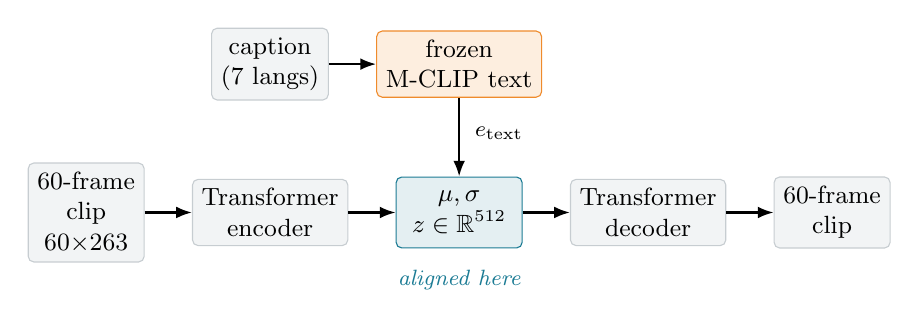
\begin{tikzpicture}[
 font=\small,
 box/.style={draw=rulegrey,fill=softgrey,rounded corners=2pt,
 minimum height=8mm,minimum width=13mm,align=center},
 lat/.style={draw=ensamblue,fill=ensamblue!12,rounded corners=2pt,
 minimum height=9mm,minimum width=16mm,align=center},
 txt/.style={draw=ensamorange,fill=ensamorange!15,rounded corners=2pt,
 minimum height=8mm,minimum width=20mm,align=center},
 arr/.style={-{Latex[length=2mm]},thick}]
% motion path
\node[box] (clip) {60-frame\\clip\\$60{\times}263$};
\node[box,right=6mm of clip] (enc) {Transformer\\encoder};
\node[lat,right=6mm of enc] (z) {$\mu,\sigma$\\$z\in\mathbb R^{512}$};
\node[box,right=6mm of z] (dec) {Transformer\\decoder};
\node[box,right=6mm of dec] (out) {60-frame\\clip};
\draw[arr] (clip)--(enc); \draw[arr] (enc)--(z);
\draw[arr] (z)--(dec); \draw[arr] (dec)--(out);
% text path
\node[txt,above=10mm of z] (text) {frozen\\M-CLIP text};
\node[box,left=6mm of text,align=center] (sent) {caption\\(7 langs)};
\draw[arr] (sent)--(text);
\draw[arr] (text.south) -- node[right=2pt,pos=0.45]{\footnotesize $e_{\text{text}}$} (z.north);
% alignment bracket
\node[below=1.5mm of z,font=\footnotesize\itshape,text=ensamblue] {aligned here};
\end{tikzpicture}
\caption{The system. A 60-frame clip is compressed by the encoder into a
single 512-dim latent $z$ and reconstructed by the decoder. A frozen
multilingual text encoder (M-CLIP, or a per-language bank) produces
$e_{\text{text}}$, which is aligned to the motion latent $\mu$ during
training. At generation time the decoder is fed $e_{\text{text}}$ in place
of $\mu$: a substitution that the base loss never optimises
(Section~\ref{sec:textrc}).}
\label{fig:arch}
\end{figure}

\section{Multilingual pipeline}

\subsection{Text encoder substitution}
The original CLIP text tower is replaced by \textbf{M-CLIP}
(XLM-RoBERTa-Large / ViT-B-32), kept \emph{frozen}, with a single
trainable $768\to512$ linear projection into the motion latent space.

\subsection{Caption translation}
HumanML3D captions are machine-translated with NLLB into six languages, \texttt{fr es pt ru zh ar}, giving seven in total with English. During
training, each clip is presented in a language sampled per clip per epoch,
so that at a fixed number of gradient steps a clip is seen in any given
language roughly $1/N$ of the time under $N$-language training. This
exposure imbalance is a confound we return to in
Section~\ref{sec:threats}.

\subsection{Per-language encoder bank}
As an alternative to the shared M-CLIP tower, we assemble a \textbf{bank of
seven frozen monolingual encoders}, each with its own trainable
$768\to512$ projection: \texttt{bert-base-uncased}~\cite{devlin2019bert},
\texttt{camembert-base}~\cite{martin2020camembert}, Spanish
BETO~\cite{canete2020beto}, Portuguese
BERTimbau~\cite{souza2020bertimbau}, Russian
RuBERT~\cite{kuratov2019rubert}, \texttt{bert-base-chinese}, and Arabic
AraBERT~\cite{antoun2020arabert}. This is \textbf{854M} frozen parameters
and \textbf{2.76M} trainable projection parameters. The supervisors'
question, whether these \emph{independently} trained projections land in
a common space, is what motivates this design.

\section{Variational formulation}
\label{sec:loss}

The training loss is a weighted sum of five terms:
\begin{equation}
L \;=\; 100\cdot\rc \;+\; 100\cdot\vel \;+\;
 \lambda_{\cos}\cdot\cos \;+\;
 \lambda_{\mathrm{CE}}\cdot\mathrm{CE} \;+\;
 \lkl\cdot\mathrm{KL}.
\label{eq:loss}
\end{equation}
Table~\ref{tab:loss} lists the terms. The $100{:}1$ weighting of
reconstruction to cosine is inherited from
MotionCLIP~\cite{tevet2022motionclip} and is \emph{not} tuned in this work;
we state this explicitly because Section~\ref{sec:cosine-fails} shows the
cosine term to be the wrong objective regardless of its weight.

\begin{table}[H]
\centering
\caption{Loss terms in Equation~\ref{eq:loss}. Default weights:
$\lrc=\lvel=100$, $\lkl=10^{-3}$; $\lambda_{\cos}$ and
$\lambda_{\mathrm{CE}}$ vary by experiment.}
\label{tab:loss}
\small
\begin{tabular}{@{}llp{8.4cm}@{}}
\toprule
Term & Symbol & Definition \\
\midrule
Reconstruction & \rc  & positional MSE, $\lVert \hat x - x\rVert^2$ \\
Velocity       & \vel & MSE on frame-to-frame differences; suppresses jitter \\
Cosine         & $\cos$ & $\mathrm{mean}\,(1-\cos(e_{\text{text}},\mu))$, matched pairs only \\
Contrastive    & CE   & InfoNCE over in-batch negatives \\
KL             & KL   & $-\tfrac12\sum(1+\log\sigma^2-\mu^2-\sigma^2)$ \\
\bottomrule
\end{tabular}
\end{table}

\section{Alignment objectives}

\subsection{Cosine similarity}
The cosine term pulls each matched text embedding and motion latent
together. Crucially it involves \emph{matched pairs only}: it contains no
negatives, so it never pushes mismatched pairs apart.

\subsection{Contrastive cross-entropy}
The contrastive term is InfoNCE~\cite{oord2018infonce} over in-batch
negatives: for each motion it raises the similarity of its own caption
above that of every other caption in the batch. The presence or absence of
negatives is the operative difference between the two objectives, and
Section~\ref{sec:cosine-fails} shows it to be decisive.

\section{Evaluation protocol}
\label{sec:eval}

\callout{\textbf{Two evaluators are used and their numbers are never
comparable.} \textbf{Evaluator~A} is the Guo/MoMask evaluator on the
\emph{official} HumanML3D test split; it reports FID~$\approx 16$ and is
used only for the M-CLIP baseline table (Section~\ref{sec:baseline}).
\textbf{Evaluator~B} (\texttt{eval\_guo\_vae\_compare\_beta05.py}) runs on
the 1{,}400-clip validation pool and reports FID~$\approx 56$--$120$; it is
used for all VAE comparisons. A number from~A and a number from~B must
never appear in the same comparison.}

\subsection{Generation metrics}
Both evaluators report \textbf{FID}~\cite{heusel2017fid} (lower is better),
\textbf{R-precision} (R@1/2/3/10, retrieval of the correct caption),
\textbf{MM-Dist} (text-to-motion feature distance, lower is better), and
\textbf{Diversity}, each over \textbf{20 replications}. One caveat must be
stated up front: \textbf{R-precision is English-only by construction}. The
Guo evaluator's text tower is a GloVe BiGRU trained on English captions, so
it can score retrieval only in English; per-language quality is therefore
assessed by FID alone.

\subsection{Latent alignment measurement}
\label{sec:align-metric}
To measure whether text and motion are aligned \emph{per sample}, we
compute cosine similarity for \textbf{matched} versus \textbf{mismatched}
text--motion pairs over 500 clips with parallel captions in all seven
languages, and report the \textbf{gap} between them. As
Section~\ref{sec:cosine-fails} shows, the \emph{mean} matched cosine alone
is actively misleading: it can be near $1.0$ while the gap, the quantity
that actually reflects alignment, is zero.

\subsection{Motion amplitude}
We introduce a diagnostic used throughout Section~\ref{sec:amplitude}: the
\textbf{mean absolute frame-to-frame difference} of a generated motion (its
overall movement), together with the difference between motions generated
for different prompts (a measure of how much the model conditions on text).

% ==================================================================
\chapter{Experiments and Results}
\label{ch:results}

This chapter is written as a sequence in which each result motivates the
next. It begins with a multilingual baseline that works, turns to a
per-language variant that appears to fail, and then, through the KL
series, discovers that the objective under which that failure was
measured is itself uninformative. The remainder builds the correct
alignment measurement, exposes the generation--discrimination trade-off and
the amplitude collapse, and closes with the controlled language comparison
that was the internship's stated question.

\section{Multilingual baseline}
\label{sec:baseline}

We first establish that multilingual conditioning works at all.
Table~\ref{tab:baseline} reports the M-CLIP variants under
\textbf{Evaluator~A} (official split, 20 replications), grouped by language
set: \emph{Latin} = \{en, fr, es, pt\}, \emph{FAR} = \{en, ru, zh, ar\}.

\begin{table}[H]
\centering
\caption{Multilingual baseline. \textbf{Evaluator~A}, official HumanML3D
test split, 20 replications. Best model value in each column in bold.}
\label{tab:baseline}
\small
\begin{tabular}{@{}lrrrrrr@{}}
\toprule
Model & FID$\downarrow$ & Diversity & R@1 & R@2 & R@3 & MM-Dist$\downarrow$ \\
\midrule
Ground truth   & 0.010  & 9.465 & 0.527 & 0.714 & 0.813 & 2.924 \\
\midrule
M-CLIP EN      & 18.013 & 7.215 & 0.128 & 0.235 & 0.327 & 6.002 \\
M-CLIP Latin   & \best{16.140} & 6.697 & \best{0.136} & \best{0.244} & \best{0.344} & \best{5.757} \\
M-CLIP FAR     & 18.046 & 7.002 & 0.111 & 0.215 & 0.304 & 6.003 \\
M-CLIP ALL     & 17.829 & 7.092 & 0.119 & 0.220 & 0.310 & 6.057 \\
\bottomrule
\end{tabular}
\end{table}

The Latin set gives the best FID ($16.14$) and the best retrieval, slightly
ahead of English-only. Multilingual conditioning is not merely tolerated;
on this split it helps. This is the encouraging result that motivated the
rest of the internship.

\section{Per-language encoders, first attempt}
\label{sec:perlang-first}

We next replaced the shared M-CLIP tower with the per-language bank (Latin
subset, four frozen backbones). Under \textbf{Evaluator~A} this appeared to
fail badly: FID $24.55$ versus $16.14$, R@1 $0.079$ versus $0.136$, and
diversity fell to ${\sim}4.0$. Reconstruction, however, was preserved
($\rc = 0.086$ versus $0.083$), so the decoder was intact and
\emph{alignment} was the casualty.

\callout{\textbf{Critical caveat, stated up front.} This comparison was
measured under the \emph{cosine} objective, which
Section~\ref{sec:cosine-fails} shows produces no per-sample alignment in
\emph{any} condition. The comparison is therefore uninformative about the
per-language encoders and is re-run under a contrastive objective in
Section~\ref{sec:textrc}, where the verdict reverses.}

This apparent failure is the origin of the supervisors' question: do the
independently trained projections share a space? Answering it
properly is what forced the alignment measurement of
Section~\ref{sec:cosine-fails}.

\section{The KL series: sampling, not regularisation}
\label{sec:kl-series}

Moving to a variational model, reconstruction immediately collapsed. The
natural suspect was the KL penalty. It is not.
Table~\ref{tab:kl-series} varies the KL treatment across four interventions
spanning two orders of magnitude of \lkl{}.

\begin{table}[H]
\centering
\caption{The KL series (sampling active). Reconstruction loss under four
interventions. Total spread $0.002$.}
\label{tab:kl-series}
\small
\begin{tabular}{@{}lr@{}}
\toprule
Configuration & \rc$\downarrow$ \\
\midrule
Deterministic autoencoder (no sampling) & \best{0.083} \\
VAE, $\lkl=10^{-5}$ & 0.524 \\
VAE, $\lkl=10^{-3}$ ($100\times$ stronger) & 0.526 \\
VAE, cosine removed (ACTOR-style) & 0.524 \\
VAE, $\lkl$ annealed over 30 epochs & 0.525 \\
\bottomrule
\end{tabular}
\end{table}

The deterministic autoencoder reconstructs at $0.083$; the moment sampling
is switched on, reconstruction jumps to ${\sim}0.52$ and \emph{stays
there}, whether the KL weight is $10^{-5}$ or $10^{-3}$, whether the cosine
term is present or removed, and whether the penalty is annealed. Four
interventions, total spread \textbf{0.002}. \textbf{Sampling is the binding
constraint, not the KL weight.}

\subsection{Why the bottleneck cannot absorb noise}
\label{sec:bottleneck}

The reason is structural. Expanding the reconstruction error to first order
in the sampling noise around $\mu$, with $z=\mu+\varepsilon$ and per-frame
decoder Jacobians $J_t=\partial\hat x_t/\partial z$:
\begin{equation}
\mathbb E_\varepsilon\lVert \hat x - x\rVert^2
\;\approx\;
\lVert \hat x(\mu)-x\rVert^2
\;+\;
\sum_{t=1}^{60}\operatorname{tr}\!\big(J_t\,\Sigma\,J_t^{\top}\big).
\label{eq:expansion}
\end{equation}
The damage term sums over \textbf{all 60 frames}, because every $J_t$
depends on the \emph{same} $z$. There is nowhere for the noise to hide: one
vector feeds the entire clip. With $K$ latents each covering a disjoint
span of frames, most $\partial\hat x_t/\partial z_k = 0$, the sum becomes
block-diagonal, and the penalty per latent falls by roughly a factor of
$K$ (Figure~\ref{fig:bottleneck}).

This also explains why ACTOR~\cite{petrovich2021actor} survives sampling
where MotionCLIP does not: ACTOR conditions on a discrete action class, so
it passes far less information through the same bottleneck and has a
lower-gain decoder, smaller $J_t$, smaller damage term.

\begin{figure}[t]
\centering
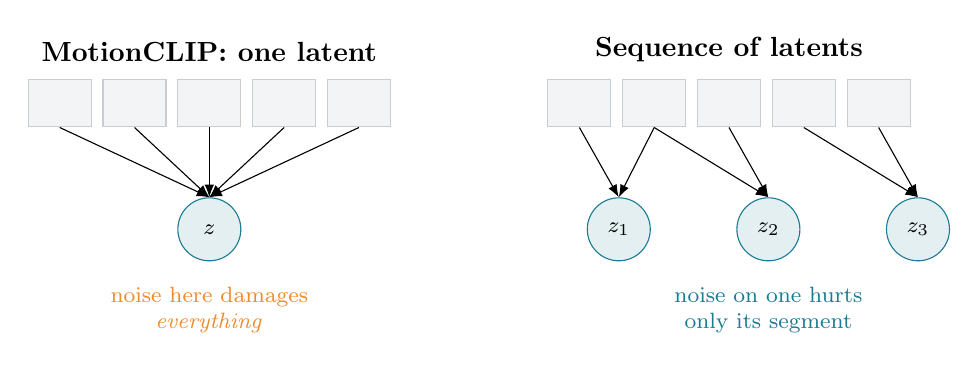
\begin{tikzpicture}[font=\footnotesize,
 fb/.style={draw=rulegrey,fill=softgrey,minimum width=8mm,minimum height=6mm},
 zt/.style={draw=ensamblue,fill=ensamblue!12,circle,minimum size=8mm},
 arr/.style={-{Latex[length=1.6mm]}}]
% LEFT: single latent
\begin{scope}
 \foreach \i in {0,...,4}
 \node[fb] (l\i) at (\i*0.95,1.6) {};
 \node[zt] (lz) at (1.9,0) {$z$};
 \foreach \i in {0,...,4} \draw[arr] (l\i.south)--(lz.north);
 \node[align=center,below=2mm of lz,text=ensamorange]
 {noise here damages\\\emph{everything}};
 \node[above=1mm of l2,font=\bfseries] {MotionCLIP: one latent};
\end{scope}
% RIGHT: sequence of latents
\begin{scope}[xshift=6.6cm]
 \foreach \i in {0,...,4}
 \node[fb] (r\i) at (\i*0.95,1.6) {};
 \node[zt] (rz0) at (0.5,0) {$z_1$};
 \node[zt] (rz1) at (2.4,0) {$z_2$};
 \node[zt] (rz2) at (4.3,0) {$z_3$};
 \draw[arr] (r0.south)--(rz0.north); \draw[arr] (r1.south)--(rz0.north);
 \draw[arr] (r1.south)--(rz1.north); \draw[arr] (r2.south)--(rz1.north);
 \draw[arr] (r3.south)--(rz2.north); \draw[arr] (r4.south)--(rz2.north);
 \node[align=center,below=2mm of rz1,text=ensamblue]
 {noise on one hurts\\only its segment};
 \node[above=1mm of r2,font=\bfseries] {Sequence of latents};
\end{scope}
\end{tikzpicture}
\caption{Why a single latent cannot absorb sampling noise. Left: all 60
frames depend on one $z$, so injected noise damages the whole clip
(Equation~\ref{eq:expansion} sums over every frame). Right: with a latent
per frame-span, most Jacobian blocks vanish and the penalty per latent
falls by roughly $K$. This is the architectural argument developed in
Section~\ref{sec:forward}.}
\label{fig:bottleneck}
\end{figure}

\section{Deterministic reconstruction, and a working VAE}
\label{sec:working-vae}

If sampling is the problem, the fix is to reconstruct from $\mu$ while
keeping the KL term. Doing so recovers reconstruction from $0.52$ to
\textbf{0.16}. The KL benchmark under \textbf{Evaluator~B}
(Table~\ref{tab:kl-bench}) then shows that KL genuinely helps generation,
and that annealing hurts in both schedules tried.

\begin{table}[H]
\centering
\caption{KL benchmark. \textbf{Evaluator~B}, 1{,}400-clip validation pool,
20 replications. KL helps; annealing hurts.}
\label{tab:kl-bench}
\small
\begin{tabular}{@{}lr@{}}
\toprule
Model & FID$\downarrow$ \\
\midrule
$\lkl=0$ & 97.633 \\
$\lkl=10^{-3}$ & \best{55.864} \\
$\lkl=10^{-3}$ + anneal over 30 epochs & 105.683 \\
$\lkl=10^{-3}$ + anneal over 5 epochs & 100.893 \\
\bottomrule
\end{tabular}
\end{table}

Annealing never had a fair test. In \texttt{reparameterize()}, sampling
activates as soon as $\lkl\neq0$, so every annealed run trained with
\emph{full-magnitude noise from epoch~1} while only the \emph{penalty} was
ramped. Separating the two variables gives Table~\ref{tab:det-then-stoch}:
train deterministically to convergence, then enable sampling.

\begin{table}[H]
\centering
\caption{Deterministic-then-stochastic training. Sampling is enabled only
after 300 deterministic epochs.}
\label{tab:det-then-stoch}
\small
\begin{tabular}{@{}lcr@{}}
\toprule
Configuration & Sampling & \rc$\downarrow$ \\
\midrule
Sampling from initialisation & on & ${\sim}0.52$ \\
Deterministic, 300 epochs & off & 0.093 \\
\quad + 10 epochs fine-tune & \best{on} & \best{0.086} \\
\bottomrule
\end{tabular}
\end{table}

\callout{\textbf{Caveat that must not be dropped.} Two variables changed
between the last two rows: sampling was enabled \emph{and} 10 further
epochs were run. The defensible claim is that \emph{sampling no longer
destroys reconstruction}, not that it improves it. The missing control, 10 further \emph{deterministic} epochs from the same checkpoint, is an
open thread (Appendix~\ref{app:expindex}). This number is also a
training-loss average; held-out confirmation across noise levels is pending
because \texttt{eval\_noise\_val100.py} loads hardcoded checkpoints and
ignored the \texttt{-{}-ckpt} override.}

\section{Noise robustness: a deliberately closed branch}
\label{sec:noise}

A tempting way to make the latent tolerate sampling is to fine-tune under
injected noise $z=\mu+\beta\varepsilon$. Reconstruction degrades smoothly
with $\beta$ (Table~\ref{tab:noise-sweep}), and fine-tuning at
$\beta=0.10$ gave a \textbf{+25.5\%} reconstruction improvement:
\textbf{92\%} of clips improved, bootstrap 95\% CI $[0.227, 0.373]$.
Statistically, this is solid.

\begin{table}[H]
\centering
\caption{Reconstruction under injected noise $z=\mu+\beta\varepsilon$.}
\label{tab:noise-sweep}
\small
\begin{tabular}{@{}lrrrrr@{}}
\toprule
$\beta$ & 0 & 0.1 & 0.25 & 0.5 & 1.0 \\
\midrule
\rc & 0.0805 & 0.0922 & 0.1621 & 0.3857 & 0.6529 \\
\bottomrule
\end{tabular}
\end{table}

Downstream, it fails. Table~\ref{tab:noise-downstream} shows the
$\beta=0.10$ fine-tune \emph{degrading} every generation metric.
Teacher distillation and encoder freezing were also tried and did not
recover it. The branch was closed.

\begin{table}[H]
\centering
\caption{Downstream effect of the $\beta=0.10$ fine-tune.
\textbf{Evaluator~B}. The auxiliary gain does not transfer.}
\label{tab:noise-downstream}
\small
\begin{tabular}{@{}lrrrr@{}}
\toprule
 & R@1 & R@3 & FID$\downarrow$ & MM-Dist$\downarrow$ \\
\midrule
original & \best{0.062} & \best{0.104} & \best{57.317} & \best{7.274} \\
$\beta=0.10$ fine-tuned & 0.031 & 0.073 & 86.774 & 9.165 \\
\bottomrule
\end{tabular}
\end{table}

\textbf{The negative transfer is the point.} An improvement on an auxiliary
metric (reconstruction under noise) does not reach generation by default;
it can actively harm it. We report the branch in full for exactly this
reason.

\section{Alignment is not what mean cosine measures}
\label{sec:cosine-fails}

We now return to the supervisors' question and measure alignment properly.
The multilingual VAE \texttt{vae-multilingual-mclip} (20 epochs) trains
cleanly: $\rc=0.1550$, $\vel=0.0594$, $\mathrm{KL}=76.77$,
text\_cosine~$=0.3127$. Its per-language FID on the multilingual pool
(\textbf{not} the official split; overall R@1 $0.042$, R@3 $0.104$, FID
$120.031$, MM-Dist $9.946$) is uniform across languages
(Table~\ref{tab:perlang-fid}), and cross-language generation drift from the
English version is tiny ($0.010$--$0.017$).

\begin{table}[H]
\centering
\caption{Per-language FID, multilingual pool (\textbf{Evaluator~B}, not the
official split). Uniform across languages.}
\label{tab:perlang-fid}
\small
\begin{tabular}{@{}rrrrrrr@{}}
\toprule
ZH & PT & RU & FR & AR & EN & ES \\
\midrule
99.777 & 106.077 & 108.627 & 108.665 & 112.151 & 114.813 & 124.894 \\
\bottomrule
\end{tabular}
\end{table}

Text-space alignment among M-CLIP embeddings (100 shared clips) is very
high: EN--FR $0.9721$, EN--ES $0.9750$, EN--PT $0.9744$, EN--RU $0.9823$,
EN--ZH $0.9762$, EN--AR $0.9700$; mean EN$\leftrightarrow$non-EN
\textbf{0.9750}, full pairwise range $0.963$--$0.982$.

\callout{\textbf{Caveat.} This last measurement is of \emph{M-CLIP}, a
frozen pretrained model. It says the text embeddings are already aligned
across languages; it says \emph{nothing} about what the VAE learned about
motion.}

The measurement that matters is matched versus mismatched similarity over
500 clips with identical motions and parallel captions
(Table~\ref{tab:matched}). Chance R@1 over 500 candidates is $0.002$.

\begin{table}[H]
\centering
\caption{Matched vs mismatched cosine, 500 clips, parallel captions
(English). The gap, not the mean, reflects alignment.}
\label{tab:matched}
\small
\begin{tabular}{@{}lrrrr@{}}
\toprule
Objective & matched & mismatched & \textbf{gap} & R@1 \\
\midrule
cosine, $\lambda=1$   & 0.7284 & 0.7282 & 0.0002 & 0.008 \\
cosine, $\lambda=100$ & 0.9777 & 0.9770 & 0.0007 & 0.012 \\
contrastive CE        & \best{0.0459} & 0.0273 & \best{0.0186} & \best{0.068} \\
\bottomrule
\end{tabular}
\end{table}

Under the cosine objective the gap is essentially zero, and R@1 sits at
chance. Raising the cosine weight $100\times$ makes it \emph{worse}: the
per-clip standard deviation \emph{fell} from $0.073$ to $0.005$, i.e.\ the
representation collapsed harder. The English-only control gives gap
$0.0000$.

\textbf{Why:} the cosine objective sums over matched pairs only. Setting
every $\mu_i$ to the mean text direction is a global optimum, the loss
falls while matched and mismatched stay identical. No weight fixes a
missing term. Note that the mean cosine \emph{falls} from $0.978$ to
$0.046$ across the fix while the model improves by an order of magnitude in
R@1; \textbf{we therefore recommend against mean cosine as a diagnostic for
this model class}, and use the matched-minus-mismatched gap throughout.

\section{Contrastive alignment across languages}
\label{sec:contrastive}

The contrastive objective produces a real, growing gap in every language.
Table~\ref{tab:gap-epochs} tracks it over training; Figure~\ref{fig:gap}
plots it.

\begin{table}[H]
\centering
\caption{Per-language alignment gap under contrastive CE, over training.
Monotonic in every language; ordering identical at every checkpoint.}
\label{tab:gap-epochs}
\small
\begin{tabular}{@{}rrrrrrrr@{}}
\toprule
epoch & en & fr & es & pt & ru & zh & ar \\
\midrule
20  & 0.0186 & 0.0175 & 0.0187 & 0.0168 & 0.0154 & 0.0134 & 0.0155 \\
40  & 0.0217 & 0.0208 & 0.0217 & 0.0201 & 0.0181 & 0.0158 & 0.0182 \\
60  & 0.0240 & 0.0232 & 0.0244 & 0.0225 & 0.0201 & 0.0174 & 0.0203 \\
80  & 0.0264 & 0.0259 & 0.0271 & 0.0249 & 0.0221 & 0.0193 & 0.0223 \\
100 & \best{0.0286} & 0.0282 & \best{0.0296} & 0.0273 & 0.0239 & 0.0207 & 0.0241 \\
\bottomrule
\end{tabular}
\end{table}

\begin{figure}[t]
\centering
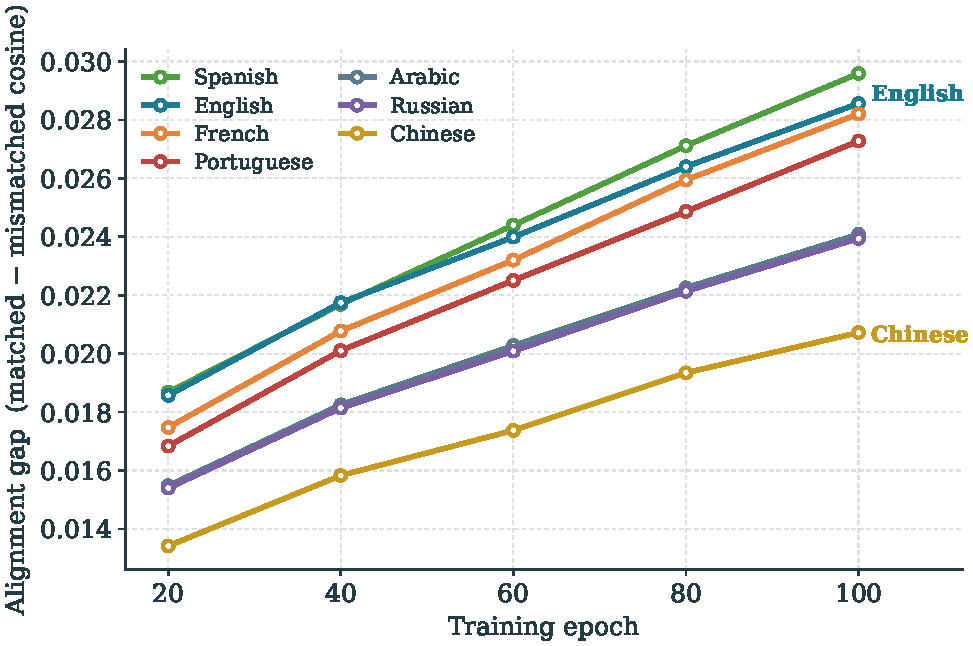
\includegraphics[width=0.78\textwidth]{figures/fig_gap_vs_epoch.pdf}
\caption{Alignment gap (matched $-$ mismatched cosine) versus training
epoch, one line per language, contrastive CE. The gap grows monotonically
in every language with no plateau. The language ordering
$\text{es}\approx\text{en}>\text{fr}>\text{pt}>\text{ar}\approx\text{ru}
>\text{zh}$ is \emph{identical at every checkpoint}: structure, not
noise. Chinese trails English by 28\% at epoch~100.}
\label{fig:gap}
\end{figure}

The ordering
$\text{es}\approx\text{en}>\text{fr}>\text{pt}>\text{ar}\approx\text{ru}>
\text{zh}$ holds at every checkpoint, and the longer 300-epoch run shows no
plateau (Appendix~\ref{app:extra}, Figure~\ref{fig:gap300}). Retrieval at
300 epochs, batch~128, is R@1 $0.068$, R@3 $0.174$, R@10 $0.340$ against
chance $0.002/0.006/0.020$. Alignment is real and well above chance.

\section{The generation--discrimination trade-off}
\label{sec:tradeoff}

The contrastive objective that fixes alignment \emph{costs} generation
quality. Table~\ref{tab:tradeoff} places the two objectives side by side.

\begin{table}[H]
\centering
\caption{The generation--discrimination trade-off. \textbf{Evaluator~B}.
Contrastive CE buys alignment and retrieval at the cost of FID.}
\label{tab:tradeoff}
\small
\begin{tabular}{@{}lrrrr@{}}
\toprule
Objective & gap (en) & R@10 & FID$\downarrow$ & Diversity \\
\midrule
cosine                & 0.0002 & 0.024 & \best{55.864} & -- \\
contrastive CE, 300 ep & \best{0.0286} & \best{0.340} & 72.902 & 0.922 \\
real motion           & -- & -- & 0.000 & 9.675 \\
\bottomrule
\end{tabular}
\end{table}

The CE-300 row in full: R@1 $0.053$, R@2 $0.098$, R@3 $0.143$, MM-Dist
$8.485$. At epoch~50 it is R@1 $0.069$, R@3 $0.177$, FID $100.781$,
Diversity $0.750$, so the diversity collapse is present \emph{early} and
is not overtraining. Rescaling text embeddings to the motion-latent norm
($20.413$ vs $9.232$) changed FID by only $2.1$ ($72.902\to70.786$) and
Diversity by $0.03$: \textbf{it is not a scale mismatch}.

\textbf{Why they dissociate:} InfoNCE constrains only the \emph{ranking} of
matched against mismatched pairs, a scale-free, direction-only property.
It never requires the latent to retain enough information to
\emph{reconstruct} a distinct motion, only enough to be
\emph{distinguishable}. A representation can be highly discriminative and
poorly decodable at the same time.

\section{Motion amplitude collapse}
\label{sec:amplitude}

The most consequential generation failure is that motions collapse toward a
near-static pose. Using the amplitude diagnostic of
Section~\ref{sec:eval}, Table~\ref{tab:amplitude} shows amplitude
\emph{falling} as models train longer and better on every other metric.

\begin{table}[H]
\centering
\caption{Motion amplitude (mean absolute frame-to-frame difference) and
between-prompt difference (walk vs jump). Better-trained models move less.}
\label{tab:amplitude}
\small
\begin{tabular}{@{}llrrr@{}}
\toprule
Model & epochs & amplitude & walk-vs-jump & ratio \\
\midrule
vae-en-mu-kl1e-3 (cosine) & 20  & \best{0.0768} & 0.1127 & 1.5 \\
vel10-test                & 60  & 0.0145 & 0.0526 & 3.6 \\
ce150-combined            & 150 & 0.0108 & 0.0409 & 3.8 \\
ce150-all                 & 150 & 0.0063 & --    & -- \\
vae-ml-sampled-ft         & 330 & 0.0044 & 0.0204 & 4.6 \\
\bottomrule
\end{tabular}
\end{table}

Three explanations are ruled out, one at a time.
\begin{enumerate}[leftmargin=*]
\item \textbf{Not a rendering artefact.} The 20-epoch checkpoint renders
 visibly different poses per prompt through the identical script.
\item \textbf{Not a text-embedding scale mismatch.} Rescaling made
 amplitude \emph{worse} ($0.01075\to0.00607$).
\item \textbf{Not the velocity weight.} At matched epochs, $\lvel=10$ gave
 slightly \emph{less} amplitude than $\lvel=100$ ($0.0145$ at 60~ep vs
 $0.0160$ at 50~ep).
\end{enumerate}

What it \emph{is}: monotonic decay within a single run, everything else
fixed (Table~\ref{tab:amp-decay}, Figure~\ref{fig:ampdecay}).

\begin{table}[H]
\centering
\caption{Amplitude decay within a single run, all else fixed.}
\label{tab:amp-decay}
\small
\begin{tabular}{@{}lrr@{}}
\toprule
epochs & ce150-combined & ce150-all \\
\midrule
50  & 0.01604 & 0.01626 \\
100 & 0.01249 & 0.00929 \\
150 & 0.01075 & 0.00626 \\
\bottomrule
\end{tabular}
\end{table}

\begin{figure}[t]
\centering
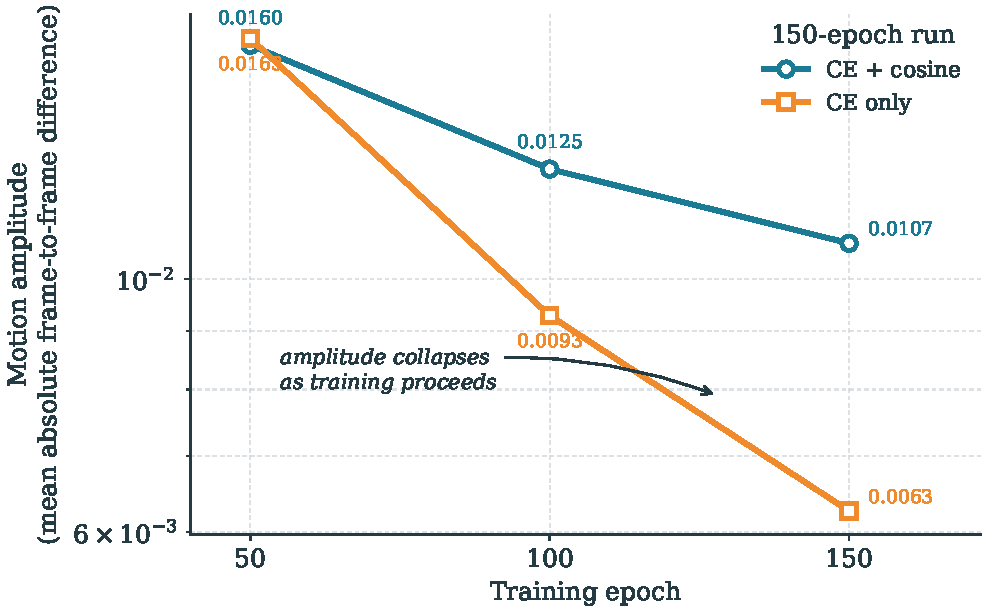
\includegraphics[width=0.68\textwidth]{figures/fig_amplitude_decay.pdf}
\caption{Motion amplitude versus training epoch for two runs (log
$y$-axis). Amplitude decays monotonically as training proceeds. The
apparently ``better'' 20-epoch model of Table~\ref{tab:amplitude} is simply
\emph{less converged}: its high amplitude is undertrained variance, not
superior motion.}
\label{fig:ampdecay}
\end{figure}

\textbf{Interpretation.} MSE reconstruction drives the decoder toward
conditional means. Averaged over pooled motion, that mean is a near-static
standing pose. Early checkpoints have not converged there yet, so they
still produce variation; the apparently better 20-epoch model is simply
less converged. This is visible directly in the generated skeletons
(Figure~\ref{fig:skeleton}), which barely move across 60 frames.

\begin{figure}[p]
\centering
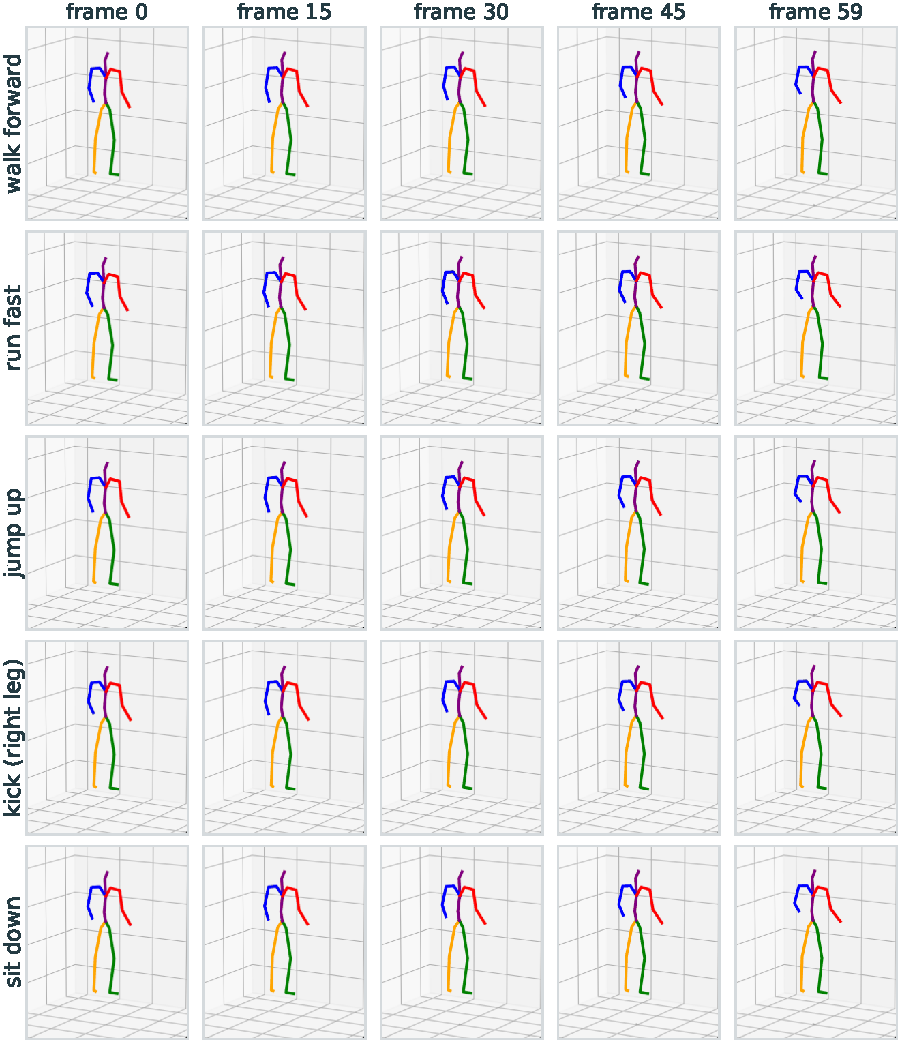
\includegraphics[width=0.90\textwidth]{figures/fig_skeleton_grid.pdf}
\caption{Generated skeletons, five prompts (rows) sampled at five
time-steps (columns) from a trained model, fixed camera and crop. Within
each row the pose barely changes across the 60 frames, and across rows the
poses are near-identical, the amplitude collapse of
Section~\ref{sec:amplitude} made visible. Frames rendered from
\texttt{gen\_vae/}.}
\label{fig:skeleton}
\end{figure}

We also verified that the \emph{encoder} is healthy: motion--motion cosine
over 200 clips spans $0.31$--$0.98$ (mean $0.61$), so it produces
well-separated latents. The collapse is on the \emph{decoder} side, and
only on the text-conditioned path.

\section{Text-conditioned reconstruction}
\label{sec:textrc}

The decoder is trained only on motion latents $\mu$, but at generation time
it is fed a \emph{text} embedding $e_{\text{text}}$
(Figure~\ref{fig:arch}). That substitution is never optimised. We add a
term that trains exactly the path generation uses:
\begin{equation}
L_{\text{text-rc}} \;=\; \lVert D(e_{\text{text}}) - x\rVert^2 .
\end{equation}
Table~\ref{tab:textrc} reports 150-epoch results.

\begin{table}[H]
\centering
\caption{Text-conditioned reconstruction and encoder choice, 150 epochs.
``walk-vs-jump'' is the between-prompt difference (conditioning strength).}
\label{tab:textrc}
\small
\begin{tabular}{@{}llcllrr@{}}
\toprule
Run & text\_rc & \lrc & encoder & amplitude & walk-vs-jump & ratio \\
\midrule
ce150-combined  & \ding{55} & 100 & M-CLIP   & 0.0108 & 0.0409 & 3.8 \\
wk-rc20         & \ding{55} & 20  & M-CLIP   & 0.0078 & 0.0376 & 4.8 \\
\textbf{wk-textrc}      & \ding{51} & 100 & M-CLIP   & 0.0042 & \best{0.2456} & \best{58} \\
\textbf{wk-textrc-rc20} & \ding{51} & 20  & M-CLIP   & 0.0030 & \best{0.2933} & \best{99} \\
wk-perlang      & \ding{55} & 100 & per-lang & \best{0.0174} & 0.0934 & 5.4 \\
wk-perlang-comb & \ding{55} & 100 & per-lang & \best{0.0192} & 0.0972 & 5.1 \\
\bottomrule
\end{tabular}
\end{table}

Two findings follow.

\textbf{Text conditioning rose 6--7$\times$} ($0.041\to0.293$): the decoder
now responds strongly to which sentence it is given. But amplitude fell
further, to $0.003$, the term rewards getting the \emph{pose} right for a
clip, not the \emph{trajectory}, since one text embedding must explain all
60 frames. The result is distinct poses per prompt with almost no movement
within each. The natural fix, applying the velocity term to the
text-conditioned output as well, to restore trajectory supervision on that
path, is proposed but not yet run (Appendix~\ref{app:expindex}).

\textbf{The per-language encoder bank gives 2--3$\times$ more amplitude}
than M-CLIP under matched settings ($0.017$--$0.019$ vs $0.006$--$0.011$).
This \emph{reverses} the apparent verdict of Section~\ref{sec:perlang-first},
which was obtained under the broken cosine objective and therefore never
measured what it appeared to.

\section{Controlled comparison: EN / Latin / FAR / ALL}
\label{sec:controlled}

The encouraging baseline of Section~\ref{sec:baseline}, where Latin FID
($16.14$) beat English-only ($18.01$), and the English degradation reported
just below are not in tension: they are read off different instruments.
Section~\ref{sec:baseline} measured FID on the \emph{official} HumanML3D
split under the cosine objective (Evaluator~A) over a longer epoch budget;
this section measures retrieval and alignment under contrastive CE at
matched compute (Evaluator~B). Same phenomenon, different instruments, and
it is the comparison in this section that is the controlled one.

Finally, the internship's stated question. All conditions are trained for
150 epochs, batch 128, contrastive CE, $\lkl=10^{-3}$, M-CLIP text encoder,
\emph{identical in every respect except the language set}. Alignment is
measured over 500 clips with parallel captions; generation via the Guo
evaluator, 20 replications.

\begin{table}[H]
\centering
\caption{Controlled language comparison. All conditions identical except
the language set. English retrieval, English alignment gap, cross-lingual
spread, and generation. Best value per column in bold.}
\label{tab:controlled}
\small
\begin{tabular}{@{}llrrrrr@{}}
\toprule
Condition & languages & en R@1 & en gap & spread & FID$\downarrow$ & Diversity \\
\midrule
EN            & en          & \best{0.610} & \best{0.0515} & 0.0398 & 67.660 & \best{1.800} \\
Latin         & en fr es pt & 0.410 & 0.0372 & 0.0253 & 95.969 & 0.668 \\
FAR           & en ru zh ar & 0.316 & 0.0336 & 0.0096 & \best{63.924} & 0.760 \\
ALL           & all 7       & 0.316 & 0.0334 & 0.0071 & 74.035 & 0.831 \\
ALL + cosine  & all 7       & 0.266 & 0.0289 & \best{0.0066} & 74.479 & 1.459 \\
real motion   & --         & 0.529 & --    & --    & 0.000 & ${\sim}9.5$ \\
\bottomrule
\end{tabular}
\end{table}

\textbf{Multilingual conditioning degrades English monotonically.} English
retrieval falls $0.610\to0.410\to0.316$ as languages are added, and
diversity drops from $1.800$ to $0.73$--$0.83$ for every multilingual
condition.\footnote{The two \texttt{eval\_all.sh} runs report English
diversity as $1.800$ and $1.798$; the evaluator has run-to-run variance of
${\sim}0.002$, which we quote as $1.800$ (Table~\ref{tab:controlled})
throughout.} This supports the \emph{lossier-shared-space} hypothesis over
the richer-supervision hypothesis: added languages induce capacity
contention rather than contributing complementary information about manner,
path, or aspect.

\callout{\textbf{The confound, restated.} At a fixed number of gradient
steps, each clip is seen in English roughly $1/N$ as often under
$N$-language training. Compute is matched; per-language \emph{exposure} is
not. Any English degradation may reflect reduced English exposure rather
than multilinguality as such (Section~\ref{sec:threats}).}

\textbf{But the degradation is not general, capacity is divided, not
lost.} Table~\ref{tab:controlled-perlang} shows each condition is best on
exactly the languages it trained on.

\begin{table}[H]
\centering
\caption{Per-language R@1 by training condition. Each condition is best on
its own languages; ALL buys the most uniform coverage at the cost of peak
performance. Best value per language in bold.}
\label{tab:controlled-perlang}
\small
\begin{tabular}{@{}lrrrrrrr@{}}
\toprule
condition & en & fr & es & pt & ru & zh & ar \\
\midrule
EN    & \best{0.610} & 0.182 & 0.188 & 0.198 & 0.118 & 0.066 & 0.084 \\
Latin & 0.410 & \best{0.388} & \best{0.430} & \best{0.438} & 0.150 & 0.100 & 0.086 \\
FAR   & 0.316 & 0.150 & 0.172 & 0.144 & \best{0.288} & \best{0.238} & \best{0.260} \\
ALL   & 0.316 & 0.272 & 0.294 & 0.298 & 0.248 & 0.172 & 0.184 \\
\bottomrule
\end{tabular}
\end{table}

\begin{figure}[ht]
\centering
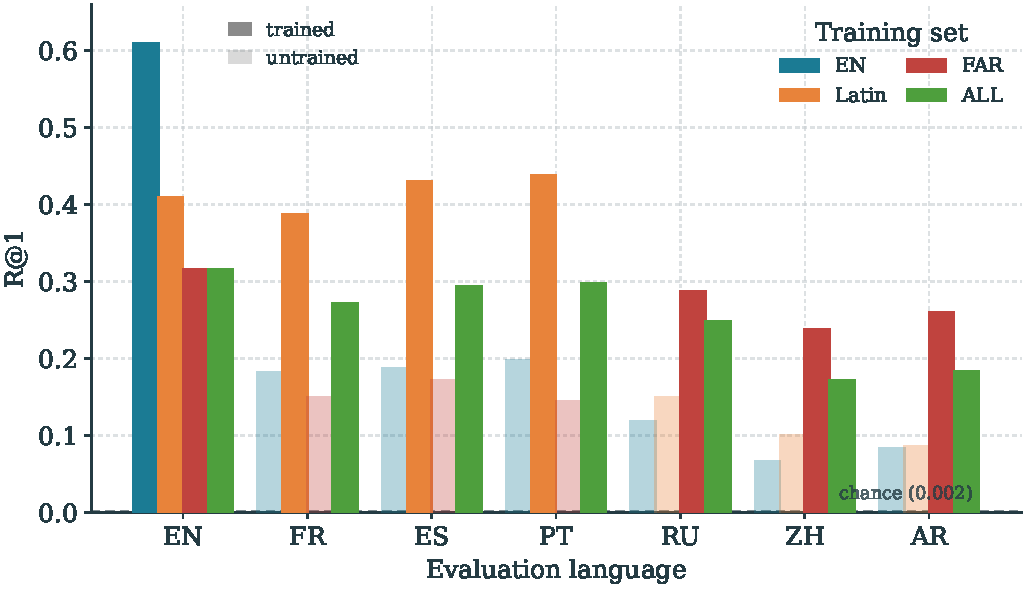
\includegraphics[width=0.74\textwidth]{figures/fig_lang_r1.pdf}
\caption{Per-language R@1 across the four language conditions. Latin lifts
fr/es/pt; FAR lifts ru/zh/ar; ALL gives the most uniform coverage. Each bar
group peaks on the languages its condition trained on, a
coverage/quality trade-off, not degradation. Dashed line: chance
($0.002$).}
\label{fig:langr1}
\end{figure}

Two secondary observations close the comparison. \textbf{Untrained
languages stay well above chance}: the Latin model reaches R@1 $0.100$ on
Chinese, $50\times$ chance, despite never seeing a Chinese caption,
which is M-CLIP's pretrained cross-lingual transfer showing through the
frozen encoder. \textbf{FAR achieves the best FID} ($63.924$) despite
weaker alignment than Latin, consistent with the dissociation of
Section~\ref{sec:tradeoff}.

\textbf{The cosine term restores diversity.} This is the clearest practical
result in the comparison. Adding the cosine term to the contrastive
objective (\emph{ALL + cosine}) roughly \emph{doubles} diversity, from
$0.73$--$0.83$ to $1.459$, second only to the English-only model, at
essentially unchanged FID ($74.479$ vs $74.035$). This is exactly the
mechanism of Section~\ref{sec:tradeoff}: contrastive CE is scale-free and
constrains only ranking, so nothing in it forces full-amplitude output; the
cosine term supplies the missing absolute constraint (raising mean
similarity from ${\sim}0.10$ to ${\sim}0.55$) while CE supplies the
per-sample separation cosine alone can never produce. \textbf{The two
objectives are complementary, and the combined loss is the recommended
configuration}: near-best diversity, the most uniform cross-lingual
coverage of any condition (spread $0.0066$), at a modest cost in peak
English retrieval.

% ==================================================================
\chapter{Discussion}
\label{ch:discussion}

\section{What the measurements support}

Four claims are supported by the evidence above. (1) In a single-latent
motion VAE, sampling, not KL strength, is the binding constraint on
reconstruction (Section~\ref{sec:kl-series}), and the first-order argument
of Section~\ref{sec:bottleneck} explains why. (2) The cosine objective
produces no per-sample alignment at any weight, while a contrastive
objective produces a real, monotone, cross-lingually structured alignment
(Sections~\ref{sec:cosine-fails}--\ref{sec:contrastive}). (3) Alignment and
generation quality dissociate (Section~\ref{sec:tradeoff}). (4) Under MSE
reconstruction, generation amplitude decays toward a mean pose
(Section~\ref{sec:amplitude}), and multilingual conditioning divides a
fixed representational budget rather than enriching it
(Section~\ref{sec:controlled}). The one clearly \emph{positive} design
recommendation is the combined CE+cosine loss, which restores diversity at
no FID cost.

\section{Threats to validity}
\label{sec:threats}

This section is deliberately blunt; it is what makes the rest credible.

\begin{itemize}[leftmargin=*]
\item \textbf{Machine-translated captions} confound translation artefacts
 with genuine typological variation. No human-authored non-English
 captions exist in this study.
\item \textbf{Per-language exposure is not matched.} Under $N$ languages,
 each clip is seen in a given language ${\sim}1/N$ as often at a fixed
 number of gradient steps. Compute is matched; exposure is not. Any
 multilingual degradation may reflect reduced English exposure rather than
 multilinguality (Section~\ref{sec:controlled}).
\item \textbf{R-precision is English-only by construction}: its text
 tower is a GloVe BiGRU trained on English. Per-language quality is
 assessed by FID alone.
\item \textbf{\lkl{} was compared against zero, not swept.}
\item \textbf{Alignment curves had not converged} at the epoch budget used
 (Figure~\ref{fig:gap}, Figure~\ref{fig:gap300}).
\item \textbf{FID values are $100\times$ above published HumanML3D
 results}; MotionCLIP is a weak generator and the VAE pool is not the
 official test split. All comparisons here are relative, not absolute.
\item \textbf{The VAE fine-tune changed two variables at once}
 (Section~\ref{sec:working-vae}); the deterministic-only control is
 outstanding.
\end{itemize}

\section{Toward a sequence of latents}
\label{sec:forward}

Every failure in Chapter~\ref{ch:results} traces to one cause: a single
512-dim latent is the wrong container for a 60-frame, multilingually
conditioned motion. The bottleneck cannot absorb sampling noise
(Equation~\ref{eq:expansion}), one text embedding cannot supply trajectory
across 60 frames (Section~\ref{sec:textrc}), and MSE regresses that single
vector toward a mean pose (Section~\ref{sec:amplitude}).

The architectural fix is a \textbf{sequence of latents}. As
Figure~\ref{fig:bottleneck} shows, distributing the clip over $K$ latents
with disjoint frame spans makes the noise-damage term block-diagonal and
lets one text embedding condition local segments rather than the whole
clip. We predict specifically that \textbf{amplitude collapse should not
appear under \emph{discrete} latents}, because quantisation prevents
regression toward a continuous conditional mean, there is no static pose
to average into. The natural test is \textbf{MoMask}~\cite{guo2024momask},
whose residual-VQ token sequence is exactly this design, conditioned on
M-CLIP text. This is the single most valuable next experiment, and it
invalidates every checkpoint produced here, which is the honest reason it
was left as the forward proposal rather than started.

% ==================================================================
\chapter{Conclusion}
\label{ch:conclusion}

The internship set out to answer whether multilingual conditioning helps or
harms 3D motion generation once capacity and compute are matched, and
whether independently trained per-language projections share a common
space. Under a controlled comparison, added languages \emph{divide} a fixed
representational budget: they improve coverage of the languages they train
on while degrading English monotonically, and they do not supply
complementary motion signal (Section~\ref{sec:controlled}).

Reaching a comparison that could be trusted required correcting the
measurement itself. Mean text--motion cosine, the obvious diagnostic, is
actively misleading for this model class: it can sit near $1.0$ while
per-sample alignment is zero (Section~\ref{sec:cosine-fails}). Replacing it
with a matched-minus-mismatched gap, and the cosine \emph{objective} with a
contrastive one, produced alignment that grows monotonically and with
stable cross-lingual structure, but at a cost in generation, because
discrimination and decodability dissociate (Section~\ref{sec:tradeoff}).
Along the way we established that sampling, not KL strength, breaks a
single-latent motion VAE (Section~\ref{sec:kl-series}), recovered a working
variational model (Section~\ref{sec:working-vae}), and diagnosed an
amplitude collapse driven by MSE reconstruction
(Section~\ref{sec:amplitude}). The one positive design result is the
combined contrastive-plus-cosine loss, which restores diversity at no FID
cost and gives the most uniform cross-lingual coverage of any condition.

What remains open is architectural and specific: move from one latent to a
sequence of discrete latents, and re-run the multilingual comparison on
MoMask with M-CLIP conditioning. Every measurement in this report points at
that experiment. The repository, the experiment index
(Appendix~\ref{app:expindex}), and the handover notes are organised so that
it can be started on day one.

% ==================================================================
\bibliographystyle{plain}
\bibliography{references}
\addcontentsline{toc}{chapter}{Bibliography}

\appendix

% ------------------------------------------------------------------
\chapter{Implementation details}
\label{app:impl}

\section{Hardware and training}
All experiments ran on a single \textbf{RTX~5090} (32~GB), shared. Training
at batch~128 runs ${\sim}32$~s/epoch. Long runs were detached with
\texttt{setsid} (not \texttt{nohup}+\texttt{disown}, which did not survive
SSH disconnects on this machine). Default training configuration: batch
128, learning rate $10^{-4}$, 60 frames, latent 512, 8 layers, GELU,
$\lrc=100$, $\lvel=100$, $\lkl=10^{-3}$.

\section{Reusable tools written during this work}
\begin{itemize}[leftmargin=*]
\item \texttt{eval\_latent\_alignment.py}, matched/mismatched gap and
 retrieval, 7 languages, per checkpoint.
\item \texttt{plot\_training\_curves.py}, parses \texttt{training.log},
 produces convergence figures.
\item \texttt{translate\_nllb.py}, NLLB caption translation into 6
 target languages.
\item Patches \texttt{patch\_vae.py}, \texttt{patch\_anneal.py},
 \texttt{patch\_mclip.py}, \texttt{patch\_ml.py},
 \texttt{patch\_perlang.py}, VAE terms, KL annealing, M-CLIP
 substitution, multilingual sampling, per-language bank.
\item \texttt{eval\_all.sh}, evaluates every \texttt{ce150-*} condition
 (alignment + generation), the source of Section~\ref{sec:controlled}.
\end{itemize}

\section{Known bugs and traps}
\label{app:bugs}
\begin{itemize}[leftmargin=*]
\item \textbf{\texttt{reparameterize()} couples \lkl{} to sampling.}
 Sampling activates as soon as $\lkl\neq0$, so every KL-annealing run
 trained with full-magnitude noise from epoch~1 while only the penalty was
 ramped. This is why annealing appeared to fail
 (Section~\ref{sec:working-vae}).
\item \textbf{Evaluation scripts hardcode checkpoints.}
 \texttt{eval\_guo\_vae\_compare\_beta05.py} and \texttt{gen\_hml.py} now
 accept \texttt{-{}-ckpt}; \texttt{eval\_noise\_val100.py} still does
 \emph{not} and ignores it.
\item \textbf{\texttt{gen\_hml.py} assumed plain CLIP} (called
 \texttt{clip.tokenize}); patched to \texttt{encode\_text\_raw} with a
 \texttt{-{}-text\_encoder} flag that \emph{must} match how the checkpoint
 was trained, or the output is silently meaningless.
\item \textbf{\texttt{logit\_scale} is missing from both custom text
 encoders}; added as a learnable (frozen) parameter to
 \texttt{mclip\_wrapper.py} and \texttt{per\_lang\_encoder.py}, without
 which the CE path crashes.
\item \textbf{Training losses are not evidence.} CE loss stayed near
 $\ln(\text{batch})$ while alignment improved $100\times$, and
 reconstruction looked healthy while motion collapsed. Always verify
 against an evaluation metric.
\end{itemize}

% ------------------------------------------------------------------
\chapter{Experiment index}
\label{app:expindex}

Every run that produced a checkpoint, the command that produced it, its key
configuration, what it tested, and its headline result. Section numbers
refer to Chapter~\ref{ch:results}. Only the final checkpoint of each run is
kept, except where the epoch progression is itself the result.

\begingroup
\scriptsize
\setlength{\tabcolsep}{4pt}
\renewcommand{\arraystretch}{1.2}
\begin{longtable}{@{}>{\raggedright\arraybackslash}p{3.2cm}%
 >{\raggedright\arraybackslash}p{3.1cm}%
 >{\raggedright\arraybackslash}p{2.7cm}%
 >{\raggedright\arraybackslash}p{4.0cm}@{}}
\toprule
\textbf{Run} & \textbf{Key config} & \textbf{Tested} & \textbf{Headline / §} \\
\midrule
\endfirsthead
\toprule
\textbf{Run} & \textbf{Key config} & \textbf{Tested} & \textbf{Headline / §} \\
\midrule
\endhead
\bottomrule
\endfoot
\cmd{ml-en} & M-CLIP, en & baseline & FID 18.013 · §\ref{sec:baseline} \\
\cmd{ml-latin} & M-CLIP, en/fr/es/pt & multilingual baseline & FID \textbf{16.140}, best · §\ref{sec:baseline} \\
\cmd{ml-far} & M-CLIP, en/ru/zh/ar & multilingual baseline & FID 18.046 · §\ref{sec:baseline} \\
\cmd{ml-all} & M-CLIP, all 7 & multilingual baseline & FID 17.829 · §\ref{sec:baseline} \\
\cmd{humanml3d-263}, \cmd{humanml3d-mclip}, \cmd{paper-model}, \cmd{my-paper-model} & original MotionCLIP & reproduction & baselines before modification (not cited) \\
\cmd{perlang-latin} & 4 frozen BERTs, cosine & per-lang encoders & FID 24.55, R@1 0.079 · §\ref{sec:perlang-first} (uninformative: cosine) \\
\cmd{vae-en-kl1e-5} & $\lkl=10^{-5}$, sampling & KL strength & rc 0.524 · §\ref{sec:kl-series} \\
\cmd{vae-en-kl1e-3} & $\lkl=10^{-3}$, sampling & KL strength & rc 0.526 · §\ref{sec:kl-series} \\
\cmd{vae-en-actor} & cosine removed & ACTOR-style & rc 0.524 · §\ref{sec:kl-series} \\
\cmd{vae-en-anneal} & anneal 30 ep & KL schedule & rc 0.525 · §\ref{sec:kl-series} \\
\cmd{vae-en-mu-kl0} & recon from $\mu$, $\lkl{=}0$ & det. recon & FID 97.633 · §\ref{sec:working-vae} \\
\cmd{vae-en-mu-kl1e-3} & recon from $\mu$ & det. recon + KL & FID \textbf{55.864} · §\ref{sec:working-vae} \\
\cmd{vae-en-mu-kl1e-3-anneal30/5} & anneal 30 / 5 ep & KL schedule & FID 105.7 / 100.9 · §\ref{sec:working-vae} \\
\cmd{vae-en-mu-beta*-ft}, \cmd{*-distill}, \cmd{*-decoderonly}, \cmd{*-musem} & $\beta$ fine-tunes & noise robustness & +25.5\% rc, FID 57.3$\to$86.8 · §\ref{sec:noise} (closed) \\
\cmd{vae-multilingual-mclip} & 7 langs, cosine & alignment & gap 0.0002 · §\ref{sec:cosine-fails} \\
\cmd{vae-ml-cos100} & cosine $\times100$ & alignment & gap 0.0007 (worse) · §\ref{sec:cosine-fails} \\
\cmd{vae-ml-ce} & CE, batch 64 & alignment & gap 0.0206 · §\ref{sec:cosine-fails} \\
\cmd{vae-ml-ce-s100} & CE, logit\_scale 100, b128 & alignment & gap 0.0186 · §\ref{sec:contrastive} \\
\cmd{vae-ml-ce-s100-e100} & CE, 5 checkpoints & gap vs epoch & monotone, Fig.~\ref{fig:gap} · §\ref{sec:contrastive} \\
\cmd{vae-ml-ce-s100-e300} & CE, 6 checkpoints & gap, generation & FID 72.902, R@10 0.340 · §\ref{sec:contrastive},\ref{sec:tradeoff} \\
\cmd{vae-ml-sampled-ft} & det.-then-sampled, 330 ep & working VAE & rc \textbf{0.086}, amp 0.0044 · §\ref{sec:working-vae},\ref{sec:amplitude} \\
\cmd{vel10-test} & $\lvel=10$ & velocity weight & amp 0.0145 · §\ref{sec:amplitude} \\
\cmd{ce150-combined} & CE+cosine, 3 ckpts & amplitude decay & amp 0.0108 · §\ref{sec:amplitude},\ref{sec:controlled} \\
\cmd{ce150-all} & CE, all 7, 3 ckpts & amplitude decay & amp 0.0063 · §\ref{sec:amplitude} \\
\cmd{wk-rc20} & $\lrc=20$ & recon weight & amp 0.0078 · §\ref{sec:textrc} \\
\cmd{wk-textrc} & text\_rc on, $\lrc{=}100$ & text-cond. recon & conditioning $\times$6, amp 0.0042 · §\ref{sec:textrc} \\
\cmd{wk-textrc-rc20} & text\_rc on, $\lrc{=}20$ & text-cond. recon & conditioning $\times$7, amp 0.0030 · §\ref{sec:textrc} \\
\cmd{wk-perlang}, \cmd{wk-perlang-comb} & per-lang bank, CE & encoder choice & amp 0.017--0.019, reverses §\ref{sec:perlang-first} · §\ref{sec:textrc} \\
\cmd{ce150-en/latin/far/all} & CE, 150 ep, language set & controlled comparison & Table~\ref{tab:controlled} · §\ref{sec:controlled} \\
\end{longtable}
\endgroup

\paragraph{Reproduction.} Each command reproduces the corresponding block
of results; \texttt{<run>} and the checkpoint epoch are filled from the
table above.

\begingroup
\small\ttfamily\setlength{\parindent}{0pt}
\newcommand{\cont}{\\[-1pt]\hspace*{2em}}
\begin{quote}
\# alignment gap + retrieval, per language\\
python eval\_latent\_alignment.py \cont
 -{}-ckpt exps/<run>/checkpoint\_XXXX.pth.tar \cont
 -{}-tag <name> -{}-n 500 -{}-text\_encoder mclip\\[4pt]
\# generation quality (evaluator B)\\
python eval\_guo\_vae\_compare\_beta05.py \cont
 -{}-model original -{}-replications 20 \cont
 -{}-device 0 -{}-ckpt exps/<run>/checkpoint\_XXXX.pth.tar\\[4pt]
\# the controlled language comparison (\S\ref{sec:controlled})\\
bash eval\_all.sh 2>\&1 | tee results\_all.log
\end{quote}
\endgroup

\paragraph{Open threads.}
(1)~Add velocity supervision to the text-conditioned path
(Section~\ref{sec:textrc}). (2)~Run 10 further \emph{deterministic} epochs
from \texttt{vae-ml-ce-s100-e300} to control the VAE fine-tune
(Section~\ref{sec:working-vae}). (3)~Sweep \lkl{}. (4)~Human-authored
non-English captions. (5)~The sequence-of-latents architecture
(Section~\ref{sec:forward}).

% ------------------------------------------------------------------
\chapter{Additional tables and figures}
\label{app:extra}

\begin{figure}[H]
\centering
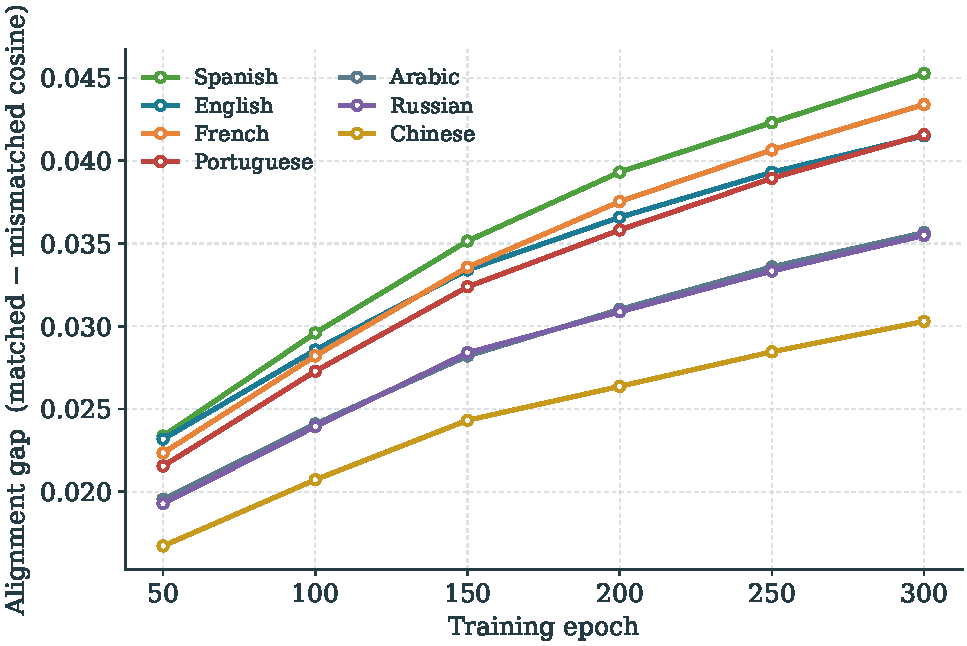
\includegraphics[width=0.80\textwidth]{figures/fig_gap_vs_epoch_300.pdf}
\caption{Alignment gap versus epoch over the long 300-epoch run, one line
per language. No plateau at 300 epochs; the cross-lingual ordering is the
same as in Figure~\ref{fig:gap}. This is the evidence for the ``curves had
not converged'' limitation in Section~\ref{sec:threats}.}
\label{fig:gap300}
\end{figure}

\begin{table}[H]
\centering
\caption{Per-language alignment gap by training condition (500 clips,
parallel captions), companion to Table~\ref{tab:controlled-perlang}.}
\label{tab:controlled-gap}
\small
\begin{tabular}{@{}lrrrrrrr@{}}
\toprule
condition & en & fr & es & pt & ru & zh & ar \\
\midrule
EN    & 0.0515 & 0.0265 & 0.0276 & 0.0249 & 0.0215 & 0.0167 & 0.0182 \\
Latin & 0.0372 & 0.0403 & 0.0420 & 0.0388 & 0.0232 & 0.0178 & 0.0206 \\
FAR   & 0.0336 & 0.0248 & 0.0262 & 0.0232 & 0.0302 & 0.0268 & 0.0316 \\
ALL   & 0.0334 & 0.0336 & 0.0351 & 0.0324 & 0.0284 & 0.0243 & 0.0282 \\
\bottomrule
\end{tabular}
\end{table}

\begin{table}[H]
\centering
\caption{Combined loss (CE + cosine), per-language matched/mismatched
cosine and gap. The cosine term raises absolute similarity to ${\sim}0.55$
while preserving a real gap.}
\label{tab:combined}
\small
\begin{tabular}{@{}lrrrrrrr@{}}
\toprule
 & en & fr & es & pt & ru & zh & ar \\
\midrule
matched    & 0.5460 & 0.5450 & 0.5460 & 0.5461 & 0.5426 & 0.5395 & 0.5430 \\
mismatched & 0.5171 & 0.5157 & 0.5153 & 0.5178 & 0.5181 & 0.5185 & 0.5187 \\
\textbf{gap} & 0.0289 & 0.0293 & 0.0307 & 0.0282 & 0.0245 & 0.0209 & 0.0243 \\
\bottomrule
\end{tabular}
\end{table}

\begin{figure}[H]
\centering
\begin{subfigure}{0.49\textwidth}
 \centering
 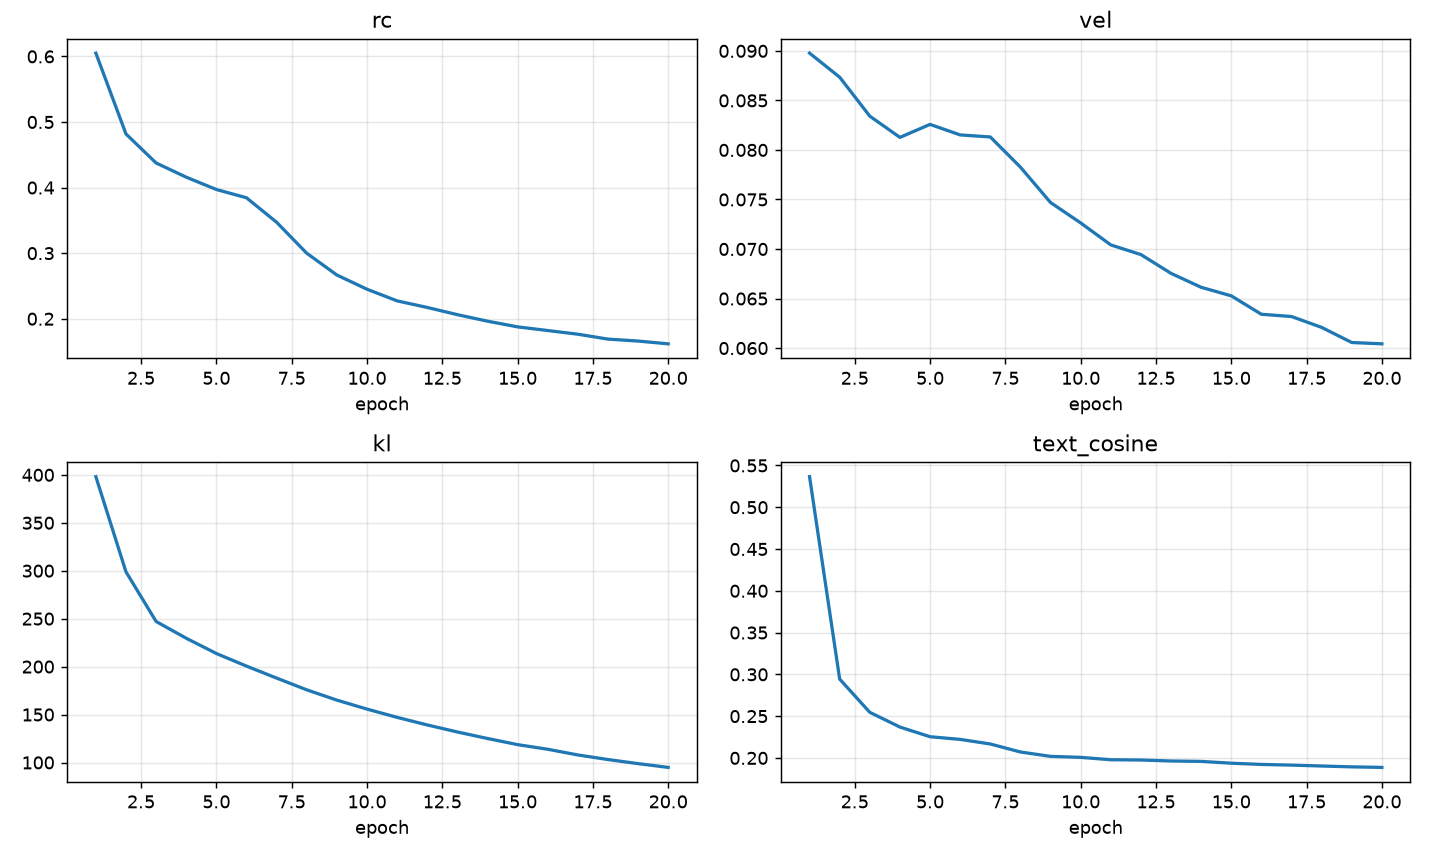
\includegraphics[width=\linewidth]{figures/curves_vae-en-mu-kl1e-3.png}
 \caption{\texttt{vae-en-mu-kl1e-3} (English).}
\end{subfigure}\hfill
\begin{subfigure}{0.49\textwidth}
 \centering
 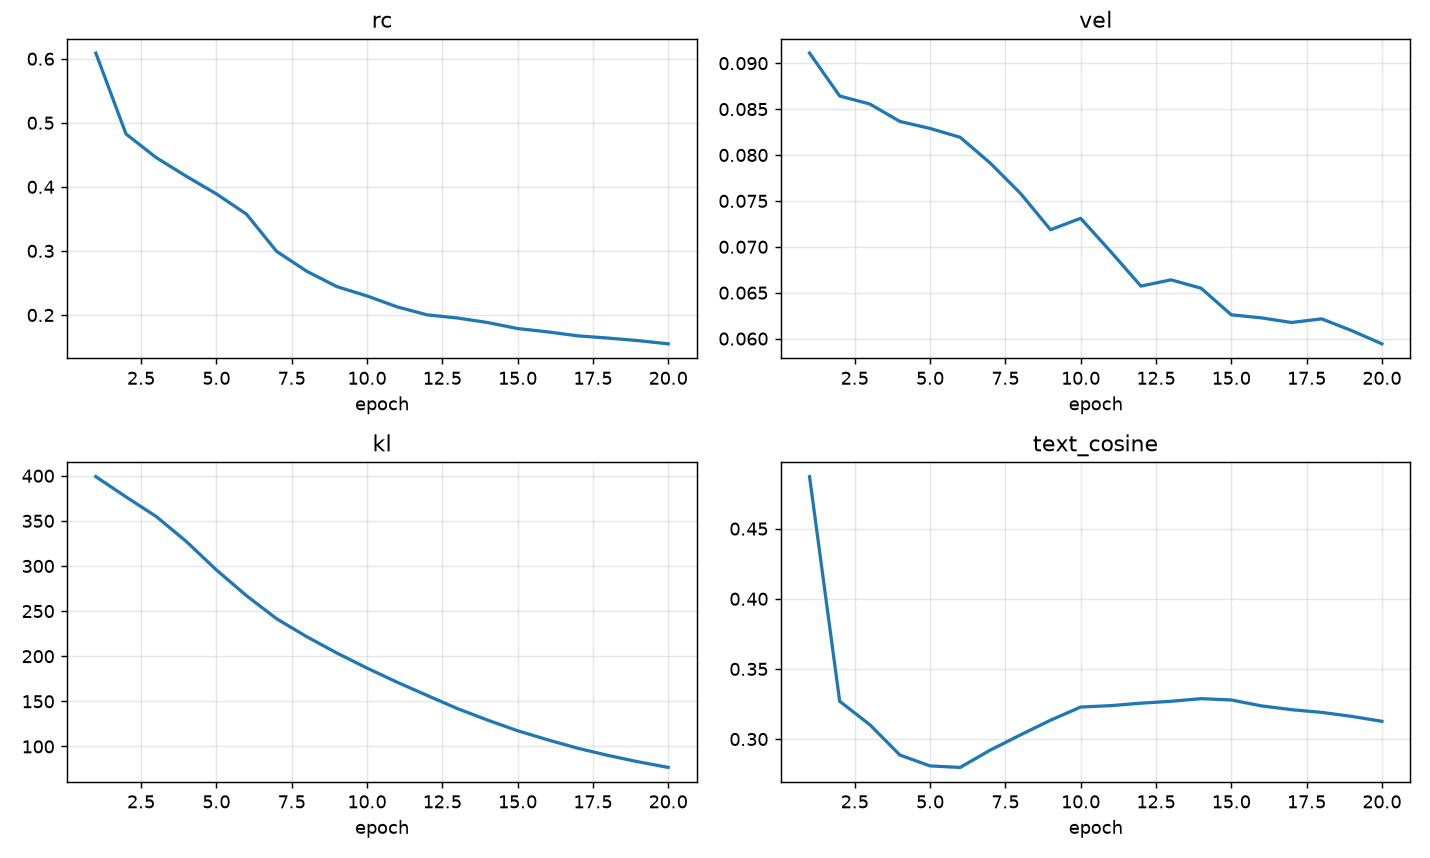
\includegraphics[width=\linewidth]{figures/curves_vae-multilingual-mclip.png}
 \caption{\texttt{vae-multilingual-mclip} (7 languages).}
\end{subfigure}
\caption{Training curves (rc, vel, KL, text\_cosine) for the English and
multilingual VAEs, produced by \texttt{plot\_training\_curves.py}.}
\label{fig:curves}
\end{figure}

\begin{figure}[H]
\centering
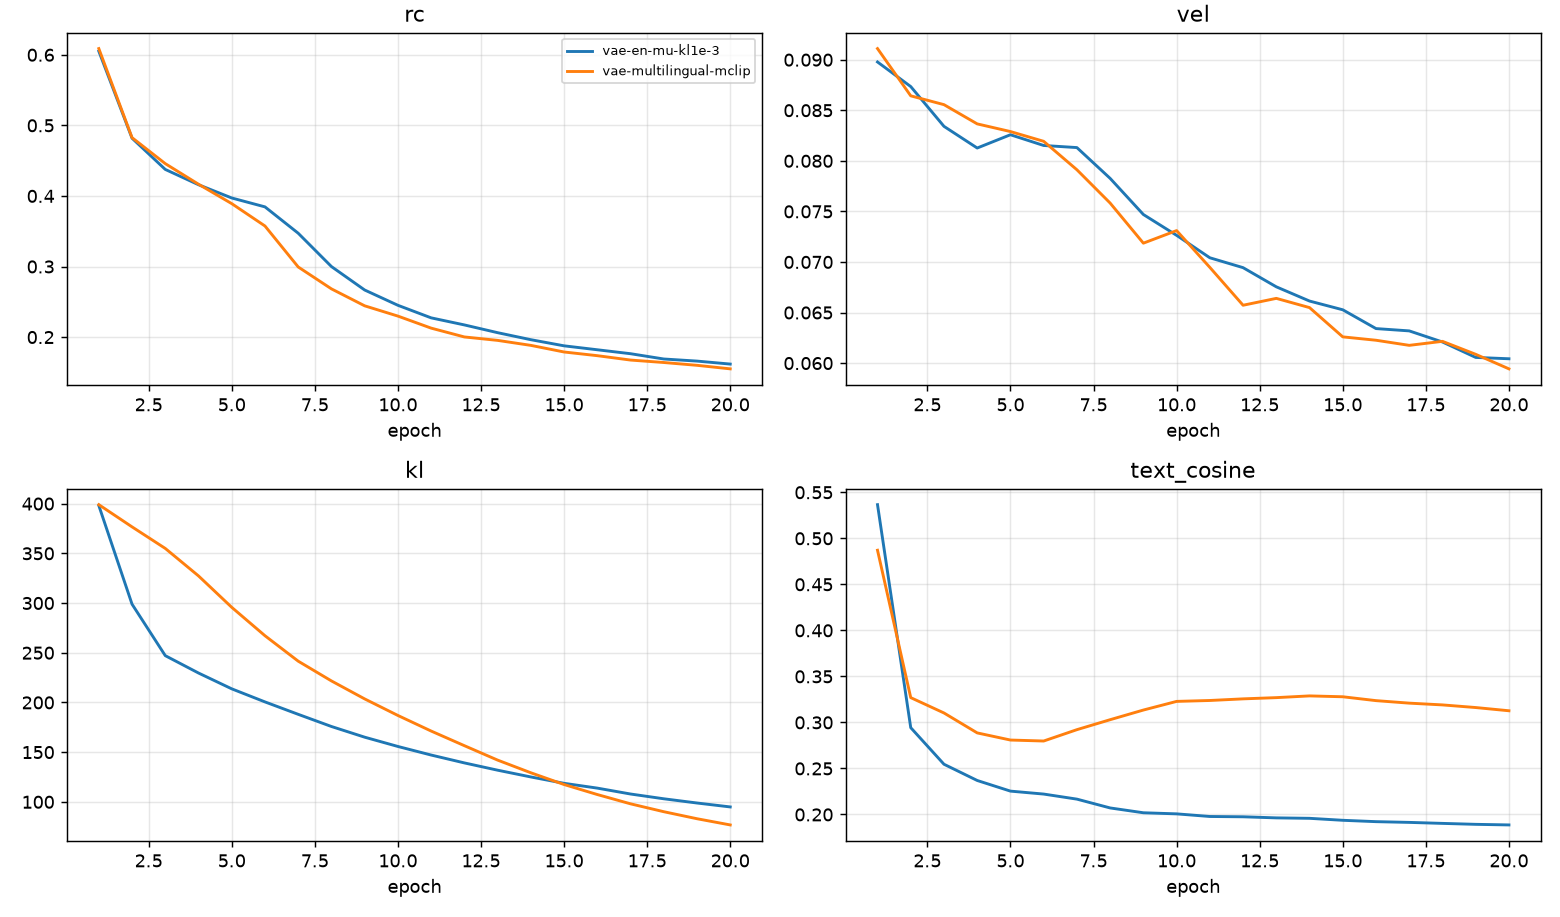
\includegraphics[width=0.78\textwidth]{figures/curves_comparison.png}
\caption{Direct overlay of the English and multilingual VAE training
curves. Reconstruction, velocity, and KL track closely; the two diverge
only in \texttt{text\_cosine}, where the multilingual model settles higher, a difference Section~\ref{sec:cosine-fails} shows to be uninformative
about per-sample alignment.}
\label{fig:curves-overlay}
\end{figure}

\begin{figure}[H]
\centering
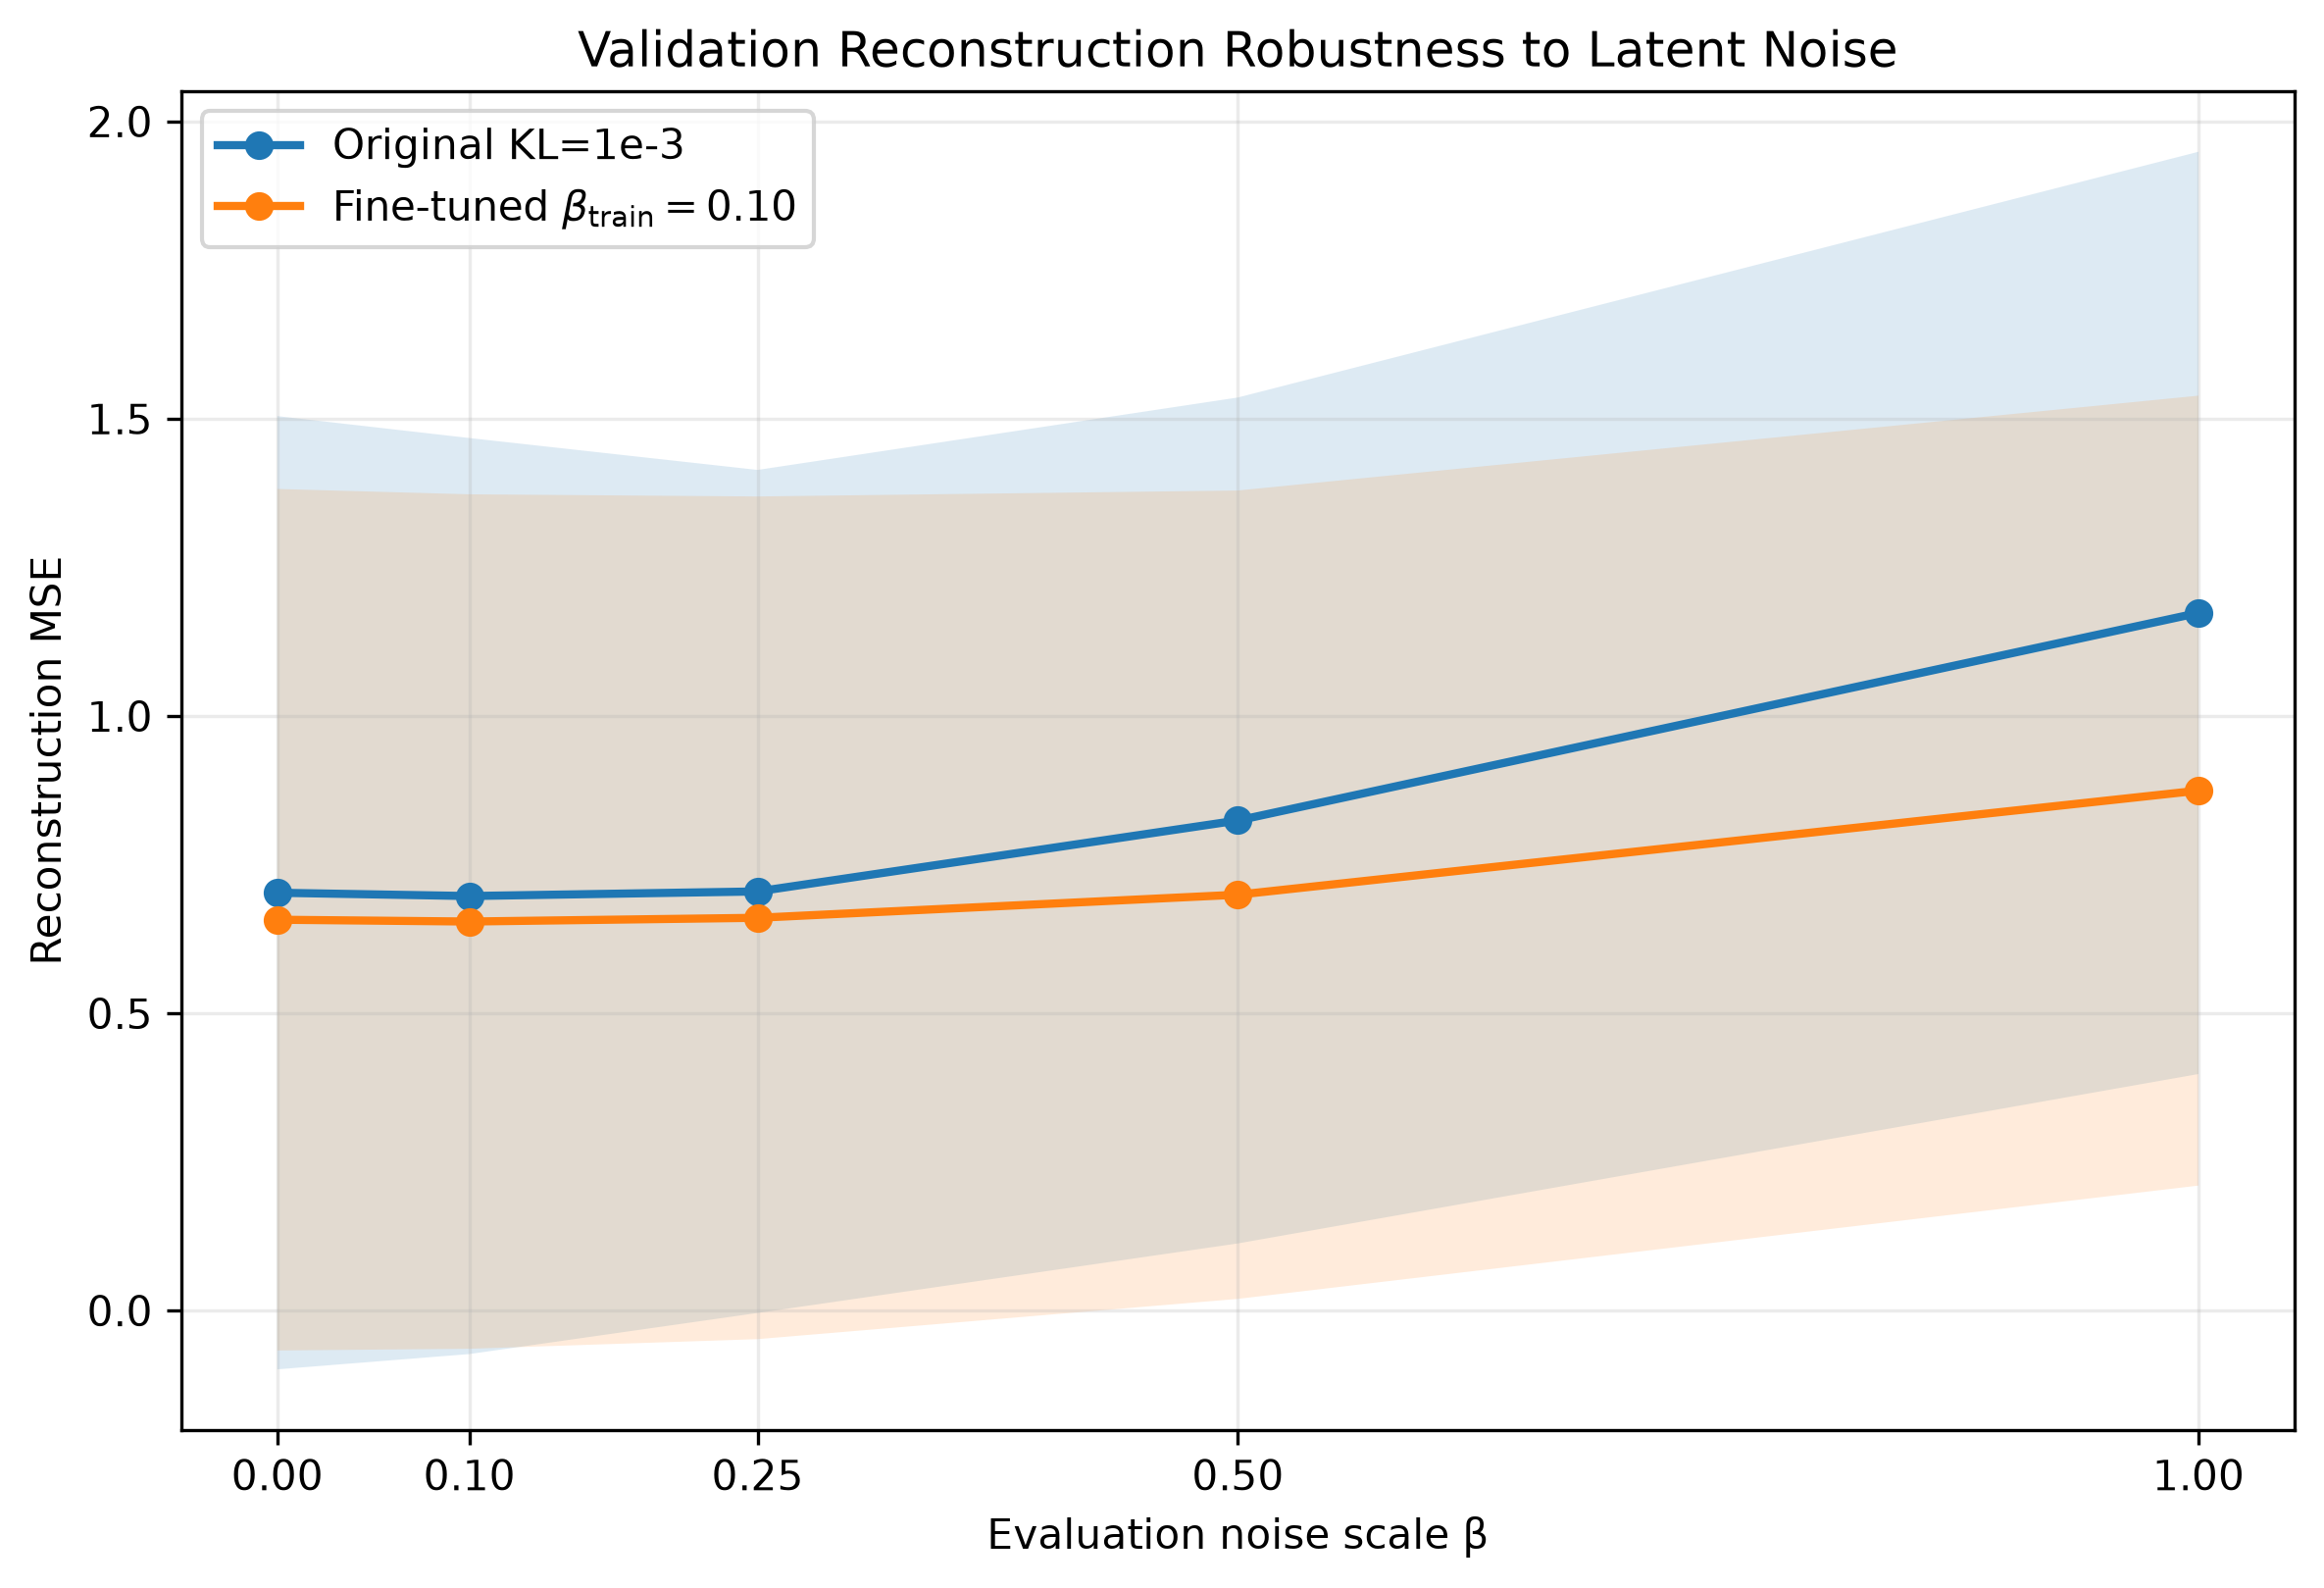
\includegraphics[width=0.72\textwidth]{figures/validation_noise_robustness.png}
\caption{Validation reconstruction under injected noise
$z=\mu+\beta\varepsilon$ for the noise-robustness branch of
Section~\ref{sec:noise}. The $\beta=0.10$ fine-tune improves reconstruction
under noise (the reported +25.5\%) but degrades generation
(Table~\ref{tab:noise-downstream}).}
\label{fig:noise}
\end{figure}

\end{document}
